%% set language, type and logo color of your thesis [german/english, bachelor/master/project, red/blue/lightblue]
\documentclass[english,master,red,footheight=14.5pt]{iRASthesis}

%% This template is derived work of KIT thesis template: https://github.com/KITrobotics/Latex_Template by Timo Rohrberg, Thorsten Haberecht and Denis Štogl
%% Adaptation by Gergely Sóti, H-KA iRAS Prof. Hein, 2021; gergely.soti@h-ka.de
%
%
% This work may be distributed and/or modified under the
% conditions of the LaTeX Project Public License, either version 1.3
% of this license or (at your option) any later version.
% The latest version of this license is in
%   http://www.latex-project.org/lppl.txt
% and version 1.3 or later is part of all distributions of LaTeX
% version 2005/12/01 or later.
%
% This work has the LPPL maintenance status `maintained'.
%
% The Current Maintainer of this work is Gergely Sóti gergely.soti@h-ka.de.
%


% language of the thesis
\title{Multi-story Navigation with\\Semantic Hierarchical Graphs}
\subtitleotherlanguage{Subtitle}
% title in the other language
\titleotherlanguage{Stockwerkübergreifender Transport mit semantischen, hierachischen Graphen}
\subtitle{Untertitel}

\author{Andreas Zachariae}
\address{My Address}
\city{7613x Karlsruhe}
\email{Andreas.Zachariae@h-ka.de}

\keywords{Keywords, of, my, Thesis, Keywords, of, my, Thesis, Keywords, of, my, Thesis, Keywords, of, my, Thesis, Keywords, of, my, Thesis, Keywords, of, my, Thesis, Keywords, of, my, Thesis}
\keywordsotherlanguge{Die, Stichw\"orter, f\"ur, meine, Arbeit, Die, Stichw\"orter, f\"ur, meine, Arbeit, Die, Stichw\"orter, f\"ur, meine, Arbeit, Die, Stichw\"orter, f\"ur, meine, Arbeit, Die, Stichw\"orter, f\"ur, meine, Arbeit}

%% Study program or a seminar/subject

%% IMPORTANT: Seminar only: If not "Seminar Intelligente Industrieroboter" uncomment this
% \nogrouplogo

%% Name of your institute (Default: IAR-IPR)
% \institute{Test}
%% Name of your faculty (Default: KIT-Fakultät für Informatik
% \KITfaculty{This is my Faculty}
%% Address of your institute (Default: Engler-Bunte-Ring 8)
% \instituteaddress{}
% %% Insitute City (Default: 76131 Karlsruhe)
% \institutecity{}

\reviewerone{Prof. Dr.-Ing. habil. Bj\"{o}rn Hein}
\reviewertwo{Dr. Ilshat Mamaev}
\editingtime{01. January 2023}{30. June 2023}

%% --------------------------------
%% | Settings for word separation |
%% --------------------------------
% Help for separation:
% In german package the following hints are additionally available:
% "- = Additional separation
% "| = Suppress ligation and possible separation (e.g. Schaf"|fell)
% "~ = Hyphenation without separation (e.g. bergauf und "~ab)
% "= = Hyphenation with separation before and after
% "" = Separation without a hyphenation (e.g. und/""oder)

% Describe separation hints here:
\hyphenation{
% Pro-to-koll-in-stan-zen
% Ma-na-ge-ment  Netz-werk-ele-men-ten
% Netz-werk Netz-werk-re-ser-vie-rung
% Netz-werk-adap-ter Fein-ju-stier-ung
% Da-ten-strom-spe-zi-fi-ka-tion Pa-ket-rumpf
% Kon-troll-in-stanz
}

%%
%% --------------------
%% |   Bibliography   |
%% --------------------
\newcommand{\mybibliographyfiles}{references}



\makeatletter
\renewcommand{\maketitle}{\bgroup\setlength{\parindent}{0pt}
  \@titlehead
\begin{flushleft}
  \vspace*{-1.5cm}
  \Huge\changefont{phv}{m}{n}
  \parbox{12cm}{
  \@title
  }
  \\
  \vspace*{0.5cm}
  \large\changefont{phv}{m}{n}
  \@subtitle  \\
  \hkadrawline \\
  \Huge\changefont{phv}{m}{n}
  \thetitleotherlanguage \\
  \vspace*{0.3cm}
  \large\changefont{phv}{m}{n}
  \thesubtitleotherlanguage  \\
  \vspace*{0.5cm}
  \Large\changefont{phv}{m}{n}
  \@author \\
  \vspace*{0.8cm}
  \large\changefont{phv}{m}{n}
  \@publishers
\end{flushleft}\egroup
\thispagestyle{empty}
}
\makeatother

% \renewcommand{\chapterpagestyle}{
% \clearscrheadfoot
% \rehead{\pagemark}
% \rohead{\pagemark}
% \ofoot{}
% }
\clearpairofpagestyles
% \rehead{\pagemark}
% \rohead{\pagemark}
% \ofoot{}

\lehead{\headmark}
\rehead*{\pagemark}
\lohead{\headmark}
\rohead*{\pagemark}
\ofoot{}

\begin{document}

% \pagestyle{plain}

\settitle
\setpdf

%% Title Page
\singlespacing
\includetitle
\includepc

\MSonehalfspacing

\includeabstract
\includeacknowledgments
\inculdetableofcontents

% \includeglossary
\inculdelistoffigures
\inculdelistoftables
\includeacronyms
\inculdelistoflistings
% \includenomenclature


\setmainpart
%% please remove following line in final version
\newacronym{iras}{iRAS}{Institute for Robotics and Autonomous Systems}
\newacronym{hka}{HKA}{University of Applied Sciences Karlsruhe}
\newacronym{ros}{ROS}{Robot Operating System}
\newacronym{ros_2}{ROS 2}{Robot Operating System 2}
\newacronym{petra}{PeTRA}{Person-Transfer Robot-Assistant}
\newacronym[plural=BTs,firstplural=Behavior Trees (BTs)]{bt}{BT}{Behavior Tree}
\newacronym[plural=FSMs,firstplural=Finite-State Machines (FSMs)]{fsm}{FSM}{Finite-State Machine}
\newacronym[plural=HFSMs,firstplural=Hierarchical Finite-State Machines (HFSMs)]{hfsm}{HFSM}{Hierarchical Finite-State Machine}
\newacronym{osrf}{OSRF}{Open Source Robotics Foundation}
\newacronym{slam}{SLAM}{Simultaneous Localization and Mapping}
\newacronym{uml}{UML}{Unified Modeling Language}
\newacronym{xml}{xml}{Extensible Markup Language}
\newacronym{lidar}{LIDAR}{Light Detection and Ranging}
\newacronym[plural=H-Graphs,firstplural=Hierarchical Graphs]{h_graph}{H-Graph}{Hierarchical Graph}
\newacronym{bmbf}{BMBF}{German Federal Ministry of Education and Research}
\newacronym{nav_2}{NAV2}{Navigation 2}
% %% ==============================
\chapter{How to use}
%% ==============================

\section{Getting Started}
If you are new to \LaTeX, please take a look at \url{https://de.overleaf.com/learn/latex/Learn_LaTeX_in_30_minutes}.

Initially you \textbf{should edit} the \texttt{my\_document\_info.tex} with important data regarding your work.

Adapt the second line of \texttt{main.tex} according to the language and type of your thesis. Regardless of language, both English and German abstracts should be written. You can also set the color of the H-KA logo (red or blue) there.

Add \textbf{content} in files in \texttt{content} folder.

Add \textbf{figures} in \texttt{figures} folder.

Add \textbf{bibliography} in the file \texttt{references.bib}.

As a useful aid in all scientific work the following book is recommended: \cite{deininger2005studien}.

Before your final submission, delete the line \texttt{\\include\{content/09-how-to-use\}} from \texttt{main.tex}.

\section{Inline lists}
My robot can:
\begin{enumerate*}[label=(\roman*)]
 \item forward and backward movements,
 \item sidewards movements,
 \item rotation along any curve in space,
 \item place of artificial forces along paths.
\end{enumerate*}

\begin{enumerate*}[label=(\arabic*),itemjoin={{; }}]
    \item the independently controllable wheels
    \item the rechargeable battery pack
    \item the Sick LMS100 laser range scanner
    \item the force-torque sensor
    \item the handlebar for controlling the robotic device
\end{enumerate*}

\url{https://ctan.math.illinois.edu/macros/latex/contrib/enumitem/enumitem.pdf}

\section{Todos}

Todo command can be used in multiple form and parameters set. You can set todos on the right side with commands:
{\small
\begin{verbatim}
\todo{Rewrite this section}
\todo[color=green]{Stuff}
\end{verbatim}
} which render as:
\todo{Rewrite this section}
\todo[color=green]{Stuff}



% \todo[due=2017-08-18]{Stuff}
% \todo[done]{Stuff}

You can also create inline todos with command:
{\small
\begin{verbatim}
\todo[inline]{Rewrite this section}
\todo[inline,color=green]{Rewrite this section}
\end{verbatim}
} which renders as:
\todo[inline]{Rewrite this section}
\todo[inline,color=green]{Rewrite this section}

One can also use command for figure placeholder with command:
{\small
\begin{verbatim}
 \missingfigure{Please add some figures}
\end{verbatim}
} which renders as:
\missingfigure{Please add some figures}


\section{Acronyms}
Please use \texttt{glossaries} package for this. See \href{https://en.wikibooks.org/wiki/LaTeX/Glossary}{\textit{documentation}}.

Example (Acronym):
{\small
\begin{spverbatim}
\newacronym{iras}{iRAS}{Institute for Applied Research - Robotics and Autonomous Systems}
\end{spverbatim}
} 
% \newacronym{iras}{iRAS}{Institute for Applied Research - Robotics and Autonomous Systems}
is used by
{\small
\begin{verbatim}
\gls{iras}
\end{verbatim}
}
% rendering as ``\gls{iras}'', on the first use and as ``\gls{iras}'' on every following use. For further feature see \href{https://en.wikibooks.org/wiki/LaTeX/Glossary}{\textit{documentation}}.


\section{SI Units}
Please use \texttt{siunitx} package for this. See:  \url{https://ctan.org/pkg/siunitx}

\section{Tables}
\begin{table}[H]
\caption{Tables have caption on top.}
\label{tab:table_caption}
\centering
\resizebox{\columnwidth}{!}{
 \begin{tabular}{| c | c | c | c |}
  \hline
  Object & Speed $[cm/s]$ & Inner LR $[cm]$ & Inner UR $[cm]$ \\ \hline \hline
  \multirow{3}{*}{\emph{Pitcher}} & real & $ n/a $ & $ 5.65 $ \\
   & $4.60$ & $3.71 \pm 0.67$ & $5.09 \pm 2.23$ \\
   & $10.64$ & $3.55 \pm 0.57$ & $6.14 \pm 0.69$ \\ \hline \hline
  \multirow{3}{*}{Cookie O} & real & $ 7.55 $ & $ 7.55 $ \\
   & $4.60$ & $6.98 \pm 0.27$ & $6.98 \pm 0.27$ \\
   & $10.64$ & $6.77 \pm 0.26$ & $6.77 \pm 0.26$ \\ \hline
 \end{tabular}
 }
\end{table}

Use \texttt{\textbackslash longtable} for tables over multiple pages. See \href{https://de.wikibooks.org/wiki/LaTeX-W%C3%B6rterbuch:_longtable_(Umgebung)}{documentation}.

\section{Figures}
\begin{figure}[H]
    \centering
    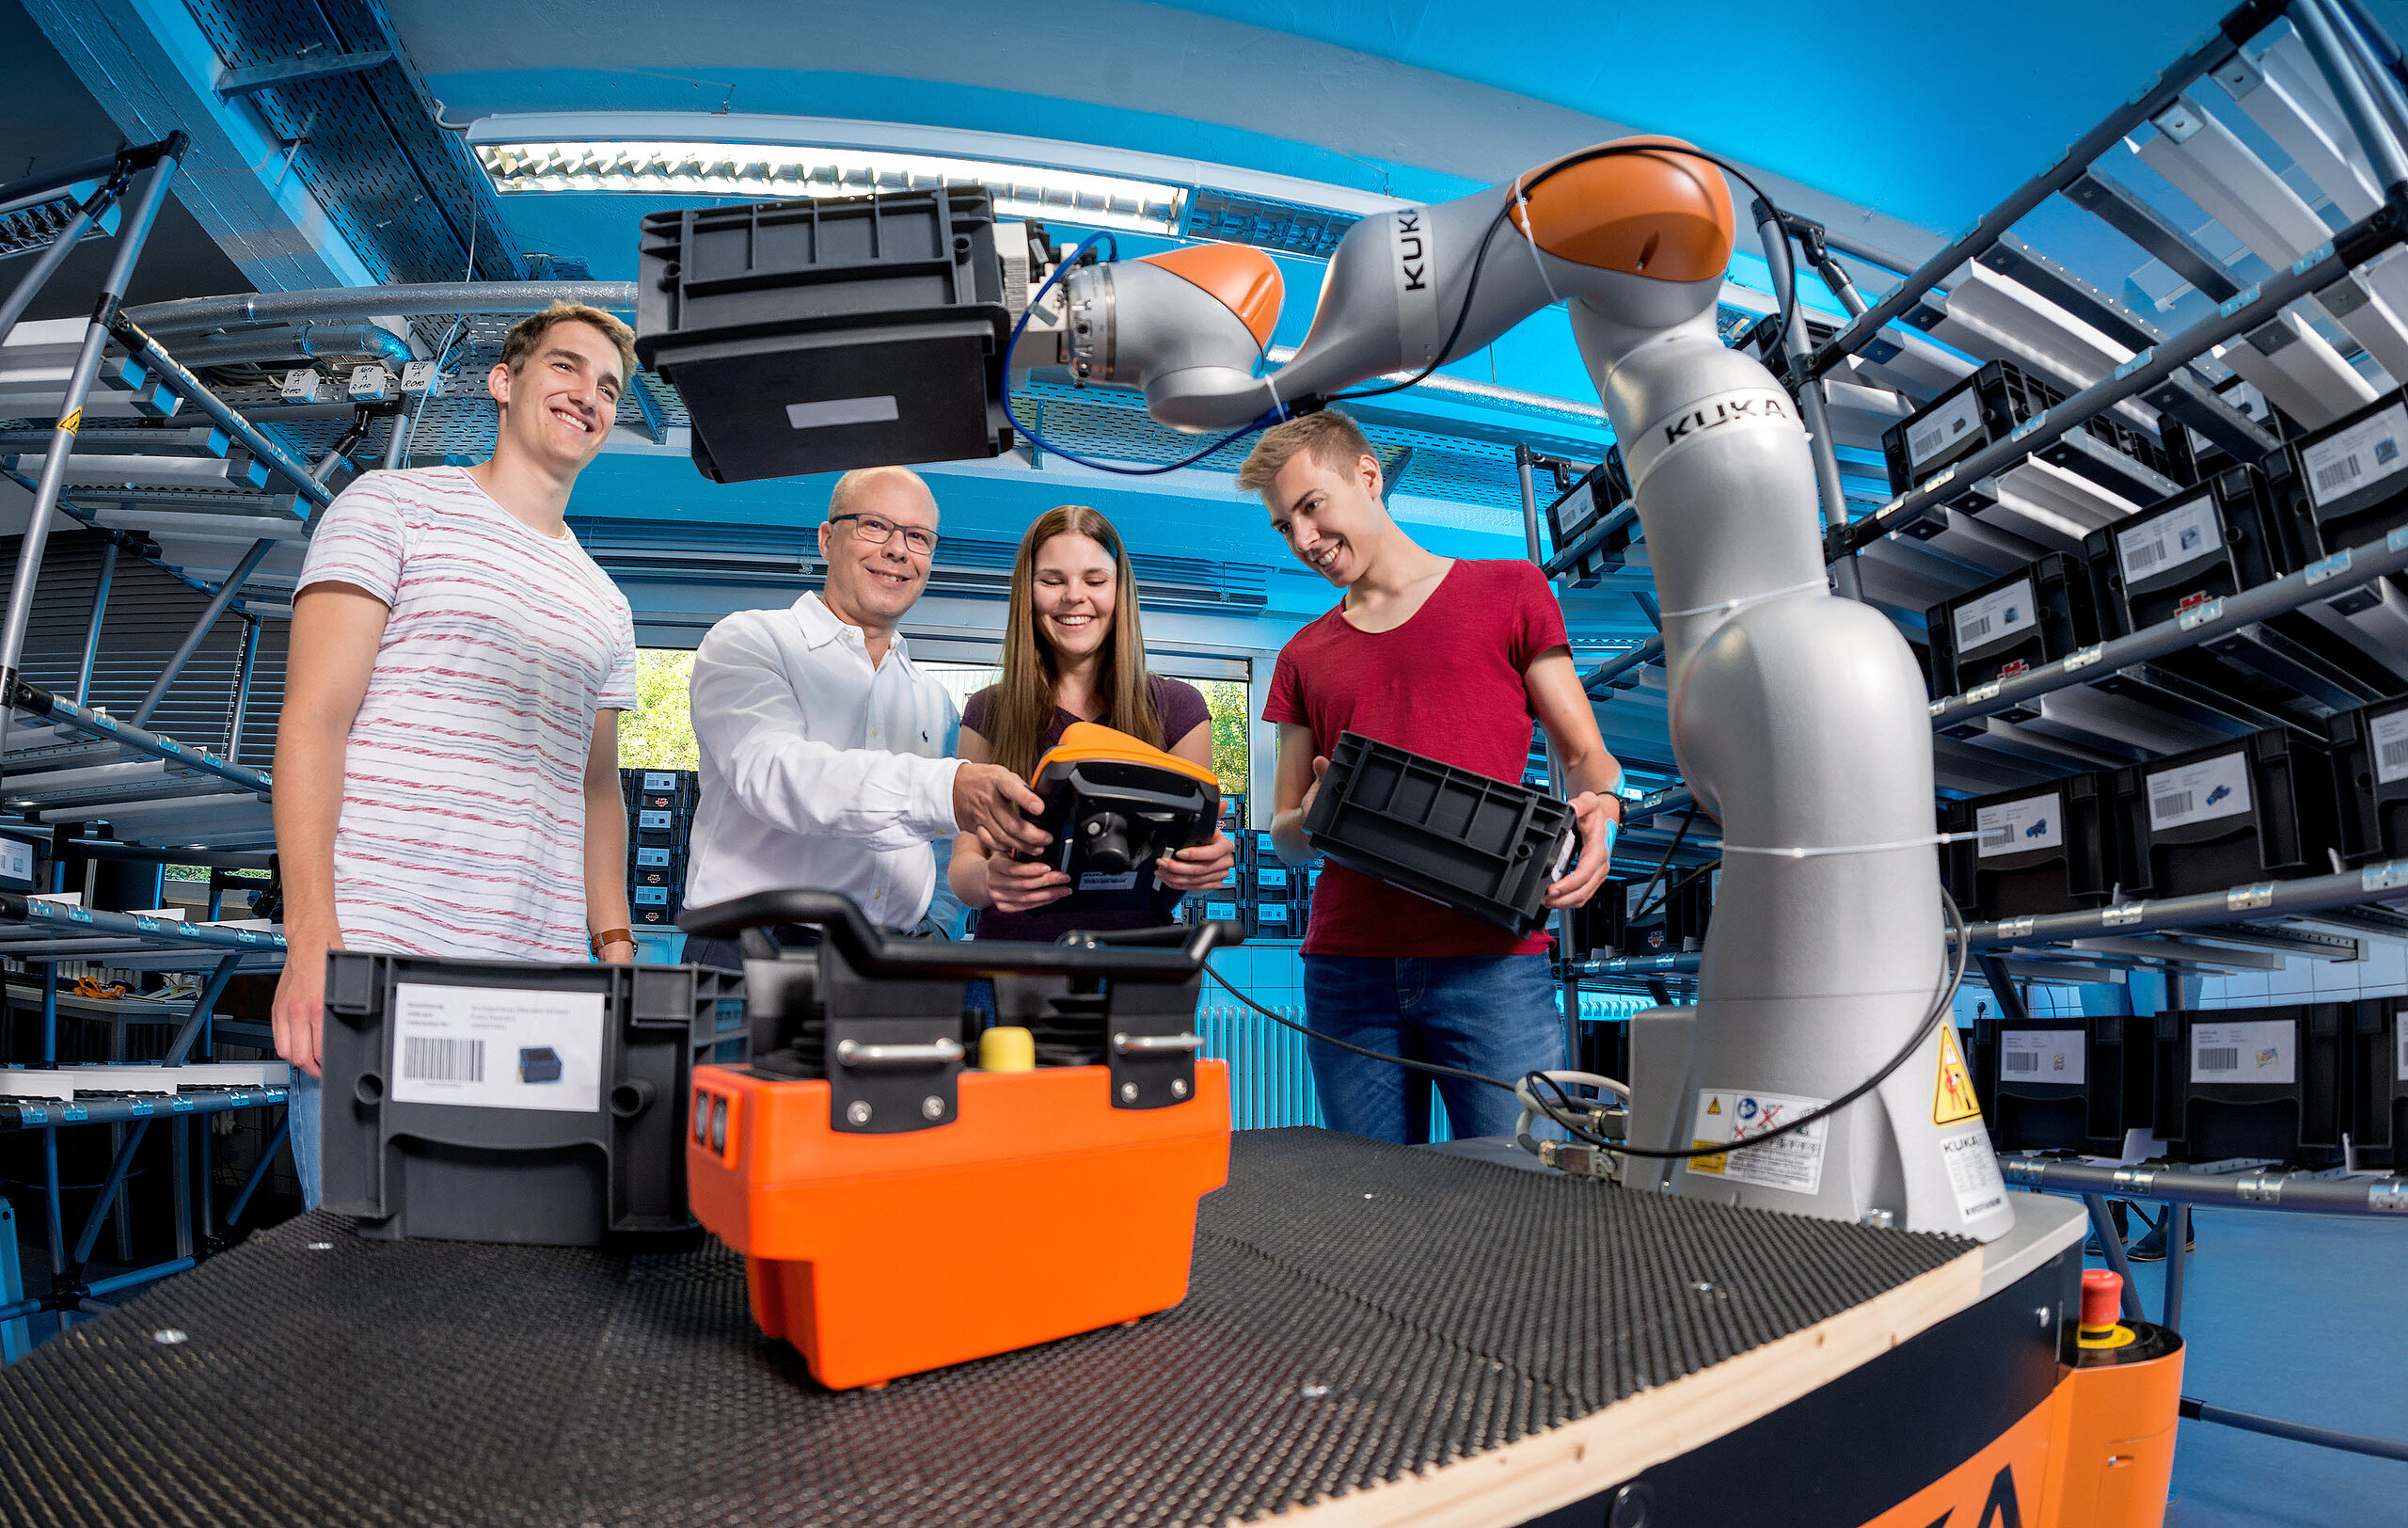
\includegraphics[width=\linewidth]{example_img}
    \caption{Figures have caption under. If you use figures from other work, do not forget to reference them \cite{deininger2005studien}.}
    \label{fig:figure_caption}
\end{figure}

\section{Subfigures}
%For more explanation see \href{https://en.wikibooks.org/wiki/LaTeX/Floats,_Figures_and_Captions#Subfloats}{Wikibooks}
\begin{figure}[H]
    \centering
    \begin{subfigure}[b]{0.3\textwidth}
        
\includegraphics[width=\textwidth]{logos/HKA_Bildmarke-v_CMYK}
        \caption{First logo}
        \label{fig:logo1}
    \end{subfigure}
    ~ %add desired spacing between images, e. g. ~, \quad, \qquad, \hfill etc.
      %(or a blank line to force the subfigure onto a new line)
    \begin{subfigure}[b]{0.3\textwidth}
        
\includegraphics[width=\textwidth]{logos/HKA_Bildmarke-v_CMYK}
        \caption{Second logo}
        \label{fig:logo2}
    \end{subfigure}
    ~ %add desired spacing between images, e. g. ~, \quad, \qquad, \hfill etc.
    %(or a blank line to force the subfigure onto a new line)
    \begin{subfigure}[b]{0.3\textwidth}
        
\includegraphics[width=\textwidth]{logos/HKA_Bildmarke-v_CMYK}
        \caption{Third logo}
        \label{fig:logo3}
    \end{subfigure}
    \caption{Pictures of Logos}\label{fig:logos}
\end{figure}


\section{Citation}

Use citations like this:
{\small
\begin{verbatim}
\cite{deininger2005studien}
\end{verbatim}
}
rendered as ``\cite{deininger2005studien}''.

\subsection{Multiple citations}
Use multiple citation like this:
{\small
\begin{verbatim}
\cite{deininger2005studien, deininger2005studien}
\end{verbatim}
}
rendered as ``\cite{deininger2005studien, deininger2005studien}''.

\section{Using Hyperlinks}
Please use the ability of PDF viewers to interpret hyperlinks\footnote{The example is from the template for the conference \href{http://www.roboticsconference.org/information/authorinfo/}{\textit{Robotic Science and Systems}}.}, specifically to allow each reference in the bibliography to be a
link to an online version of the reference.
As an example, if you were to cite ``Passive Dynamic Walking''
\cite{McGeer01041990}, the entry in the bibtex would read:

{\tiny
\begin{spverbatim}
@article{McGeer01041990,
  author = {McGeer, Tad},
  title = {\href{http://ijr.sagepub.com/content/9/2/62.abstract}{Passive Dynamic Walking}},
  volume = {9},
  number = {2},
  pages = {62-82},
  year = {1990},
  doi = {10.1177/027836499000900206},
  URL = {http://ijr.sagepub.com/content/9/2/62.abstract},
  eprint = {http://ijr.sagepub.com/content/9/2/62.full.pdf+html},
  journal = {The International Journal of Robotics Research}
}
\end{spverbatim}
}
\noindent
and the entry in the compiled PDF would look like:

\def\tmplabel#1{[#1]}

\begin{enumerate}
\item[\tmplabel{1}] Tad McGeer. \href{http://ijr.sagepub.com/content/9/2/62.abstract}{Passive Dynamic
Walking}. {\em The International Journal of Robotics Research}, 9(2):62--82,
1990.
\end{enumerate}
%
where the title of the article is a link that takes you to the article on IJRR's website.


Also use this for adding links into text as done in the \footnotemark[1]. For more information see documentation on \href{https://de.wikibooks.org/wiki/LaTeX-W%C3%B6rterbuch:_hyperref}{wikibooks}. The \texttt{hyperref} package is already configured for this document in \texttt{document\_setup.tex} file.


\section{Equations}
Use numbered equations:
\begin{equation} \label{equ:equ}
  m \cdot \ddot{x}(t) + d \cdot \dot{x}(t) = F(t)
\end{equation}

Reference equations, figures, tables or anything with a label by 

\begin{spverbatim}
\ref{label_name}
\end{spverbatim}
e.g. Equation \ref{equ:equ}

\section{Code or Algorithms}

\lstset{language=C++, caption={Pseudocode einer \textit{Sequence} mit \textit{N} Kindern}, label={lst:Pseudocode Sequence}}
\begin{lstlisting}
for i %\textbf{from}% 1 %\textbf{to}% %\textit{N}% do
    child_status = tick(child[i])
    if child_status == %\textit{Running}%
        return %\textit{Running}%
    if child_status == %\textit{Failure}%
        return %\textit{Failure}%
return %\textit{Success}%
\end{lstlisting}

\lstset{language=Python, caption={Python Skript zum Definieren eines Greifverhaltens}, label={lst:Python Greifverhalten}}
\begin{lstlisting}
def GraspObject(self):
    rospy.loginfo("Grasping an object from table...") # prepare for grasping
    myhandle = self.sss.Move("arm","pregrasp",False)
    self.sss.Move("sdh","cylopen")
    myhandle.wait()
    # grasp the object
    self.sss.Move("arm","grasp")
    self.sss.Move("sdh","cylclosed")
    # put object on tray
    myhandle = self.sss.Move("arm","grasp-to-tablet",False)
    self.sss.Move("tray","up")
    myhandle.wait()
    self.sss.Move("sdh","cylopen")
    # draw arm back to folded position
    myhandle = self.sss.Move("arm","tablet-to-folded",False)
    self.sss.Move("sdh","cylclosed")
    myhandle.wait()
\end{lstlisting}


%% ==============================
\chapter{Introduction}
\label{sec:introduction}
%% ==============================
Questions to ask:
\begin{enumerate}
    \item What is your research topic? (From wide to narrow scope)
    \item What is the research problem or gap in the field that this work aims to address?
    \item Why is this problem or gap important?
    \item What are the research questions or hypotheses? 
    \item What is the scope of your work? (What are the limitations?)
    \item How is the following work structured?
\end{enumerate}

\begin{enumerate}
    \item General field of path planning for mobile robots
    \item Problem of path planning in multi-floor environments
    \item Shared human-robot spaces
    \item Research question: How to plan in a multi-floor environment? And how to drive in public spaces with service robots?
    \item Significance: Many use cases in public spaces in large, complex hierarchical environments like hospitals.
    \item Development of a global planner plugin for straight and predictable paths in multi-floor environments.
    \item Structure of the thesis
\end{enumerate}

%% ==============================
\section{Motivation}
\label{sec:motivation}
%% ==============================
The research area of autonomous mobile robotics deals with all sub-areas that are necessary to ensure the required degree of autonomy and mobility for specific tasks. In addition to navigation and manipulation, this also includes the perception of the environment as well as the internal state. Autonomous mobile robots form a combination of the disciplines of electrical engineering, mechanical engineering and computer science. Computer science in particular is rapidly driving current developments. Complex algorithms for localisation and navigation enable the necessary mobility. Artificial intelligence offers robust methods for image processing, object recognition and voice control through neural networks and machine learning. According to the market research company Gartner, autonomous robotics is the most important strategic technological trend of 2019 \cite{cearley_gartner_2018} and number eight in 2020 \cite{david_cearley_gartner_2019} In recent years it has only been superseded by new developments in the field of AI. The market for professional service robots is growing rapidly. According to the International Federation of Robotics, the number of professional service robots sold in 2021 grew by 37 \% to a total of 121,000 units \cite{international_federation_of_robotics_world_2022}. The largest are of application is transportation and logistics. These are robots that mostly operate in strictly defined spaces separated from humans, for example robots for material logistics in warehouses or production facilities.

Especially in the application area of service robotics in shared human-robot spaces, tasks are becoming increasingly complex. The best-known are household robots for consumers that, for example, take care of vacuuming or mow the lawn. However, more extensive tasks such as support in everyday life by folding the laundry \cite{srivastava_tractability_2015} or assisting in the kitchen \cite{becker_pr2_2011}, can now also be taken over by assistance robots. The professional application of service robots is mostly limited to isolated tasks without the need to interact with humans. There are a few start-ups which are trying to establish service robots in public spaces as well \cite{kittmann_let_2015}. However, the development of service robots for public spaces is still in its infancy. The main reason for this is the complexity of the tasks and the environment. In addition to the technical challenges, there are also legal and ethical issues that need to be addressed.

%% ==============================
\section{Problem Statement}
\label{sec:problem_statement}
%% ==============================
Mobile robots are increasingly being used in large environments, such as hospitals, to improve efficiency and reduce human workload. However, navigating over multiple stories poses a significant challenge for mobile robots, as it requires a planner that can account for complex spatial configurations and still find the shortest path. Moreover, the planned path must be straight, deterministic and predictable for humans who could be walking in the same space as the robot. Therefore, the specific research problem addressed in this thesis is the development of a planner that can enable a mobile robot to navigate over multiple stories in complex environments, while ensuring a straight and human-predictable path. 

The ability to navigate over multiple stories is important for mobile robots in large, complex environments, as it can significantly increase their utility and effectiveness. For instance, in hospitals, mobile robots could be used for tasks such as delivering medicines, transporting equipment, or guiding patients and visitors. Although for specific use-cases proprietary solutions exist, the lack of an open-source planner for multi-floor navigation is a major bottleneck in the development of mobile robots for service applications. Moreover, the need for a straight and human-predictable path is essential for ensuring safety and reducing the risk of collisions or accidents in shared human-robot spaces.

The two main research questions addressed in this thesis are:
\begin{enumerate}
    \item How to navigate in complex multi-floor environments?
    \item How to plan paths that are straight and human-predictable?
\end{enumerate}

The scope of this work is limited to the development of a planner that plans a priori with previously collected information, as opposed to a controller that follows the planned path and adapts to dynamic obstacles. The main assumption is that a map of the entire environment has been previously recorded and provides a complete representation of the plannable space.

%% ==============================
\section{Use case PeTRA}
\label{sec:use_case}
%% ==============================
The use case of this work is a mobile robot that is used to support staff with patient logistics in care facilities. This includes tasks such as delivering medicines and transporting a patient to examinations. This work is part of the \gls{petra} research project, which is funded by the \gls{bmbf} \cite{bmbf-internetredaktion_bekanntmachung_2018} and developed at the \gls{iras} of the \gls{hka}.

The daily routine in a hospital includes transporting patients from ward to examination. This manual transport is mostly performed by trained nurses, who are can not perform nursing activities while they are absent from the ward. To reduce transfer time, patients are moved through the hospital in beds, even though some of them would be able to walk by themselves. This transfer method neither promotes the patients' mobility nor allows them to decide for themselves whether and how they want to walk. "\Gls{petra} is designed to relieve caregivers of time-consuming and labor-intensive patient transport and give them more time for qualitative care" \cite{petra-konsortium_personen-transfer_2022}. To achieve this goal, an autonomous mobile robot was developed in collaboration with industry partners and three hospitals. \Gls{petra} offers different transfer modes, to adapt to each patients need, see figure  \ref{fig:multi_mobility_methods}. Autonomous patient transport is realized with sensory coupling for free walking or with the support of a rollator (center) and a modular platform for wheelchairs (left). This platform is used for safe wheelchair transport and can be coupled. In addition, an integrated robotic arm performs service tasks (right). These include, for example, the transport of drugs or blood samples between the storage area and the wards..

\begin{figure}[h]
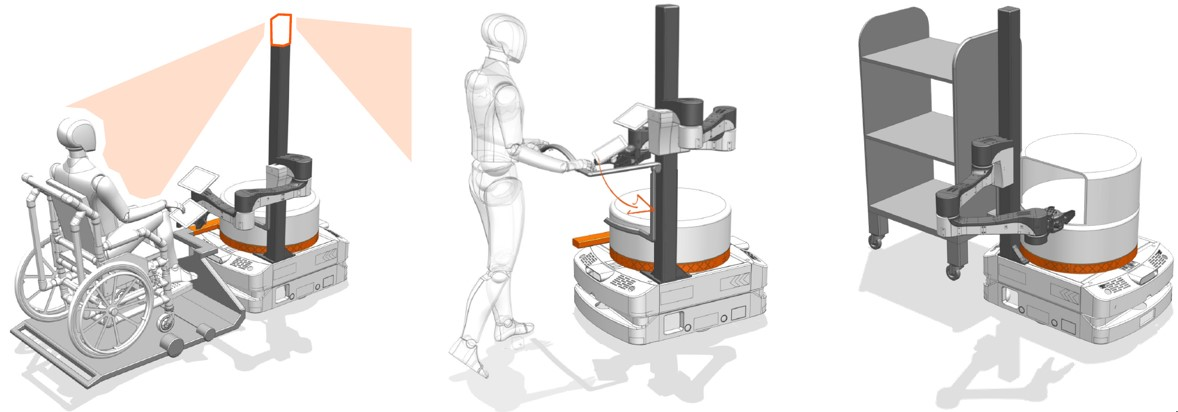
\includegraphics[width=\textwidth]{figures/20_state_of_the_art/PeTRA_transport_modes.jpg}
\caption[]{Multi-mobility methods of PeTRA: Wheelchair transport (left), sensory coupling (center) and material transport (right).}
\centering
\label{fig:multi_mobility_methods}
\end{figure}
To demonstrate the feasibility and economic viability of autonomous transports in hospitals \gls{petra} needs to be able to carry out jobs between arbitrary locations in this complex environment. This work enables \gls{petra} to navigate over multiple floors while following a predictable path.

%% ==============================
\section{Structure of this Thesis}
\label{sec:structure}
%% ==============================
The following work is structured as follows: Chapter \ref{sec:state_of_the_art} provides an overview of the state of the art in the field of multi-floor path planning for mobile robots. It also discusses the limitations of existing approaches. Chapter \ref{sec:methods} describes the methodology used to address the research questions. The concept of the graph-based planner is presented in Chapter \ref{sec:concept} followed by the implementation in Chapter \ref{sec:implementation}. This shows the approaches of creating a graph from a previously recorded map. Chapter \ref{sec:results} presents the results of the work. Chapter \ref{sec:discussion} discusses the results and provides recommendations for future work. Chapter \ref{sec:conclusion} concludes the thesis.
%% ==============================
\chapter{State of the art}
\label{sec:state_of_the_art}
%% ==============================
Questions to ask:
\begin{enumerate}
    \item What is generally known about the topic? (relevant theory)
    \item What are the most important (recent) existing works in the field related to the research problem? 
    \item Provide a comprehensive review of the relevant literature, including key theories, concepts, and previous studies that inform your research question.
    \item What are the limitations or gaps in the existing works that this work aims to address? 
    \item How does this work build upon or differ from existing works? 
    \item What are the main research approaches or techniques used in the field, and how do they relate to this work? 
    \item What are the main challenges or open questions in the field? 
\end{enumerate}

General theory:
\begin{enumerate}
    \item Path planning
    \item Astar, RRT, Dijkstra, PRM
    \item Hierarchical graphs
    \item ROS2 Nav Stack
    \item OpenRMF
    \item Behavior Trees
\end{enumerate}

The following overview of the state of the art consist of four main parts:
\begin{enumerate}
    \item The general theory of path planning in mobile robotics is presented. This includes the most common algorithms for path planning, and their applications in real robotic systems. (Chapter \ref{sec:path_planning}).
    \item The recent approaches to hierarchical planning in complex multi-floor environments are presented. This shows the existing approaches to the first research question: "How to navigate in complex multi-floor environments?" (Chapter \ref{sec:hierarchical_planning}).
    \item The recent approaches to straight path planning are presented. This shows the existing approaches to the second research question: "How to plan paths that are straight, deterministic and human-predictable?" (Chapter \ref{sec:straight_paths}).
    \item The research gap and limitations of the state of the art is summarized (Chapter \ref{sec:research_gap}).
\end{enumerate}

%% ==============================
\section{General Path Planning for Mobile Robots}
\label{sec:path_planning}
%% ==============================

The general approach to path planning in mobile robotics is a two-layered architecture which can be seen in Figure \ref{fig:path_planning_two_layered_architecture}. The first layer is the global path planning layer. It is responsible for finding a path from the start to the goal position in a previously known static environment. The second layer is the collision avoidance also known as local path planner or controller. It is responsible for avoiding dynamic obstacles that prevent the global path from being executed. For both layers there are different approaches as open source solutions available. This concept is further explained with the example in chapter \ref{sec:navigation_stack}.

\begin{figure}[h]
    \centering
    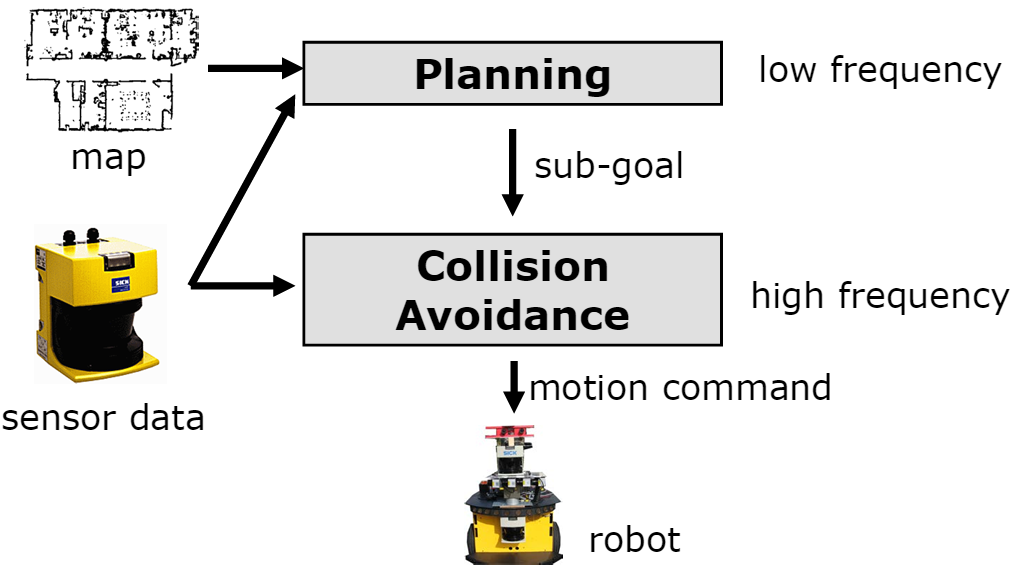
\includegraphics[width=0.75\textwidth]{figures/20_state_of_the_art/path_planning_two_layered_architecture.png}
    \caption[The two layered architecture for mobile robot path planning]{The two layered architecture for mobile robot path planning (Source: \cite{burgard_introduction_2021})}
    \label{fig:path_planning_two_layered_architecture}
\end{figure}
The scope of this work is limited to extending the capabilities of the global planner for multiple floors. The collision avoidance is solved with existing algorithms. The following sections will give an overview of the most common existing global planner algorithms. 



%% ==============================
\subsection{Path Planning Algorithms}
Planning a path is a major challenge in robotics and is necessary for mobility. The path from the robot's current location to the goal can be planned in two ways: deterministically or probabilistically. Deterministic planners use algorithms that always deliver the same results with the same input. Probabilistic planners, on the other hand, are based on randomness and produce different results for the same input. The map on which deterministic planners are based is usually discretised into a lattice. In an informed search, heuristics can be used to tell whether one grid field is closer to the target configuration than another. According to Burgard in \cite{XXBurgard}, the performance of a search algorithm is measured in four different ways:
\begin{enumerate}
    \item Completeness:
    Does the algorithm find the solution if there is one?
    \item Optimality:
    Is the solution the best of all possible solutions in terms of path cost?
    \item Time complexity:
    How long does it take to find a solution?
    \item Space complexity:
    How much memory is needed to perform the search?
\end{enumerate}

%% ==============================
\subsection{The Robot Operating System 2}
\begin{displayquote}
    \enquote{The \acrfull{ros} is a framework for writing robot software. It is a collection of tools, libraries, and conventions that aim to simplify the task of creating
    complex and robust robot behavior across a wide variety of robotic platforms.} \cite{quigley_programming_2015}
\end{displayquote}
    
\begin{figure}[h]
    \centering
    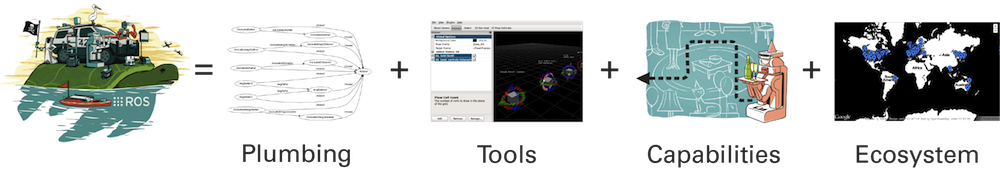
\includegraphics[width=1\textwidth]{figures/20_state_of_the_art/ros_equation.png}
    \caption[The ROS equation]{The ROS equation: ROS = Plumbing + Tools + Capabilities + Community (Source: \cite{open_robotics_ros_2020})}
    \label{fig:ros_equation}
\end{figure}

The development of \gls{ros} began in 2007 as part of the Stanford AI Robot Project (STAIR) and was mainly driven by Willow Garage. There it was used as the basis for the Personal Robot 2 (PR2), but has been intended from the start as an open-source platform for a wide range of robotic applications. By now, the development is being driven forward by Open Robotics. The founders, Brian Gerkey and Morgan Quigley, have also published a comprehensive book to make it easier to get started with \gls{ros} \cite{quigley_programming_2015}. The \gls{ros} ecosystem consists of much more than pure code; it thrives on a large community and the exchange of ready-to-use packages, which is described by the '\gls{ros} equation' in Figure \ref{fig:ros_equation}. Since 2011, \gls{ros} has has left the earth for the International Space Station with NASA's Robonaut 2 \cite{koubaa_ros_2016}. Due to the rapidly growing community and increasing application in industry, an improved version was developed and released in December 2018 as \gls{ros_2}. The main difference is the focus on real-time applications and the use of the industry standard 'Data Distribution Service' (DDS) for the communication of distributed systems \cite{macenski_robot_2022}.

Nodes are the basis of the distributed network of an \gls{ros} application. The nodes are executed independently of each other and communicate with each other via defined interfaces. This offers the advantage that applications can be built up modular, can be easily exchanged, and can be used in conjunction with other applications. A node can contain several topics, services or actions with which data can be exchanged with other nodes. Different nodes in a \gls{ros} application can be executed on different hardware. A collection of nodes that perform a completed function are grouped together as a package and shared by many developers around the world. A combination of related packages with a version history and managed documentation is called a stack. For example, there is the Navigation Stack, which contains all the functions needed to move the robot safely from A to B. This includes algorithms for localisation and path planning as well as the processing of sensor data for obstacle avoidance and mapping.

\begin{figure}[h]
    \centering
    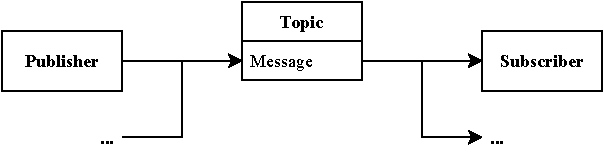
\includegraphics[width=0.75\textwidth]{figures/20_state_of_the_art/topics.pdf}
    \caption{The structure of a ROS topic}
    \label{fig:topics}
\end{figure}

The individual nodes communicate through message channels about a specific topic. This communication is designed for distributed systems and enables a many-to-many (n:m) cardinality. This means that each node can act as a publisher or subscriber of any topic, see Figure \ref{fig:topics}. The content of the message is defined by a .msg file as the interface.

\begin{figure}[h]
    \centering
    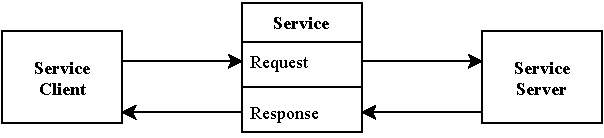
\includegraphics[width=0.75\textwidth]{figures/20_state_of_the_art/services.pdf}
    \caption{The structure of a ROS service}
    \label{fig:services}
\end{figure}

Services are based on the call-and-response model. This means that, unlike topics, messages are not unilaterally sent into the network. Instead, a request is made from a client to a server, and a response is sent back, as illustrated in Figure \ref{fig:services}. The structure resembles a function call, where parameters are passed and a return value is expected. The data types are defined in the corresponding .srv file. This type of communication is particularly useful for computations performed by another node \cite[p. 51]{quigley_programming_2015}. Services can be executed synchronously or asynchronously. In a synchronous call, the calling node blocks the thread until the response arrives. Synchronous calls should only be used when the service requires a short, finite amount of time for computation. Asynchronous calls are implemented by providing a predefined function (callback) that is automatically invoked by \gls{ros} when the service response is received. This allows other code to be executed in the node as long as it does not depend on the service result.

\begin{figure}[h]
    \centering
    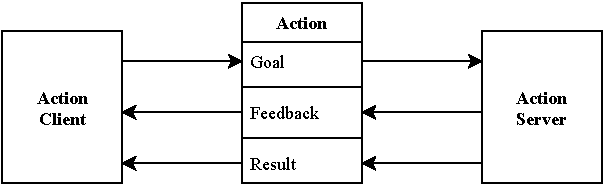
\includegraphics[width=0.75\textwidth]{figures/20_state_of_the_art/actions.pdf}
    \caption{The structure of a ROS action}
    \label{fig:actions}
\end{figure}

Actions have been a fixed component of the communication vocabulary since \gls{ros_2}. They are designed for the asynchronous execution of long-duration actions. In addition to the concept of services, actions allow for the exchange of feedback data during execution. Furthermore, actions provide the ability to cancel their execution. An action client sends a request (goal) to the action server, which can either accept or reject the goal. During execution, a feedback callback is invoked at the client until the result is received and processed. Actions offer a high-level communication protocol, as shown in Figure \ref{fig:actions}. A good example of the application of actions is robot movement towards a specific goal. The task should occur asynchronously and can vary in duration. Through the feedback mechanism, information about the current position of the robot can be communicated, and if the goal becomes outdated, the action can be canceled. The interface of an action for navigation is defined by an .action file, as depicted in Algorithm \ref{lst:navigatetopose.action}.

\lstset{language=python, caption={NavigateToPose.action, definition of an action from type 'NavigateToPose'}, label={lst:navigatetopose.action}}
\begin{lstlisting}
# goal
geometry_msgs/PoseStamped pose
-%{}%-%{}%-
# result
std_msgs/Empty result
-%{}%-%{}%-
# feedback
geometry_msgs/PoseStamped current_pose
builtin_interfaces/Duration navigation_time
int16 number_of_recoveries
float32 distance_remaining
\end{lstlisting}
    
%% ==============================
\subsection{The Navigation Stack in ROS2}
\label{sec:navigation_stack}

\begin{displayquote}
    \enquote{Nav2 is the professionally supported spiritual successor of the ROS Navigation Stack. This project seeks to find a safe way to have a mobile robot move to complete complex tasks through many types of environments and classes of robot kinematics. Not only can it move from Point A to Point B, but it can have intermediary poses, and represent other types of tasks like object following and more. Nav2 is a production-grade and high-quality navigation framework trusted by 50+ companies worldwide.} \cite{steve_macenski_navigation_2020}
\end{displayquote}

The \gls{nav_2} stack for \gls{ros_2} is a comprehensive framework for the development of new planner algorithms. The planner developed in this work is based on the \gls{nav_2} stack and is written as an exchangeable plugin for the existing structure. With its server and plugin layout \gls{nav_2} supports custom planner, controller behavior and smoother plugins. In Figure \ref{fig:nav2_architecture} the architecture of \gls{nav_2} is shown. It follows the classic two-layered architecture for path planning seen in Figure \ref{fig:path_planning_two_layered_architecture}. The planner server provides the global path planning on a known map and the controller server offers algorithms for following this path with dynamic obstacle avoidance. The necessary inputs for this system are the map, the odometry of the robot wheels and the sensor data from lidars or cameras. With this information the localization can calculate the most likely position of the robot in the map. The planner plans a path from this current position to the goal. In a control loop, the controller tries to reduce the error between the current position and the planned path. The output of the controller is a velocity command for the robot. The velocity command is then executed by the robot's motor controller.

\begin{figure}[h]
    \centering
    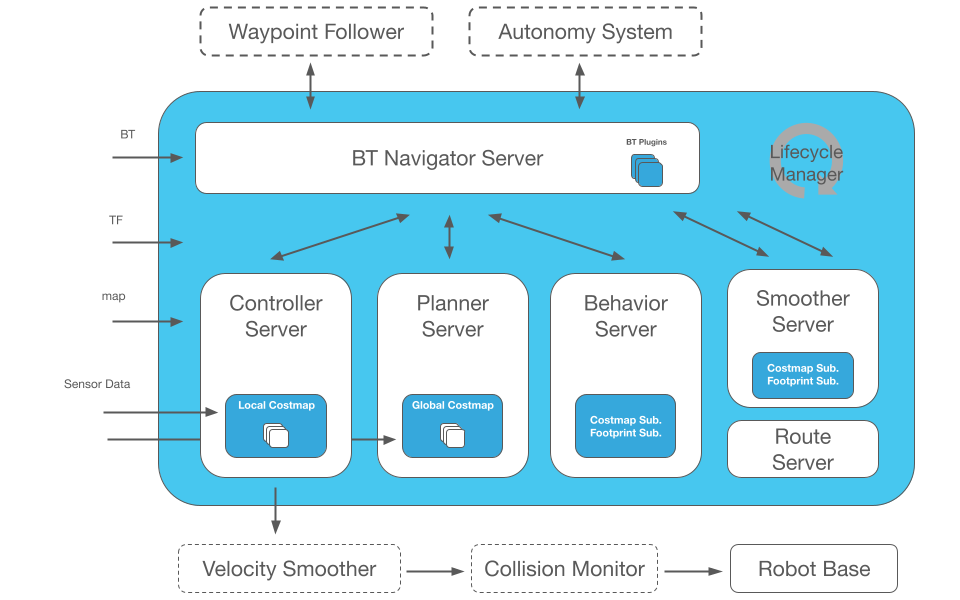
\includegraphics[width=\textwidth]{figures/20_state_of_the_art/nav2_architecture.png}
    \caption[The architecture of the \gls{nav_2} stack]{The architecture of the \gls{nav_2} stack (Source: \cite{steve_macenski_navigation_2020})}
    \label{fig:nav2_architecture}
\end{figure}

In this work a new planner, capable of planning in complex multi-floor environments, is developed. The algorithm is implemented as a plugin for the planner server. The rest of the \gls{nav_2} pipeline is used with existing packages.

%% ==============================
\subsection{Behavior Trees for Navigation}

\gls{nav_2} is the most prominent example of \glspl{bt} in robotics and especially for navigation. It uses \glspl{bt} to create customized and intelligent navigation behavior by orchestrating many independent modular servers. The default \gls{bt} for executing a navigation request to a specific goal is shown in Figure \ref{fig:nav2_bt}. It shows the actual planner, an A* algorithm, on the left side which is triggered every second (1 Hz). All other named actions are recovery behaviors which are used to clear the costmaps and reorient the robot if it gets stuck. To understand the symbolic language of the \gls{bt} the single elements are explained in the following section.

\begin{figure}[h]
    \centering
    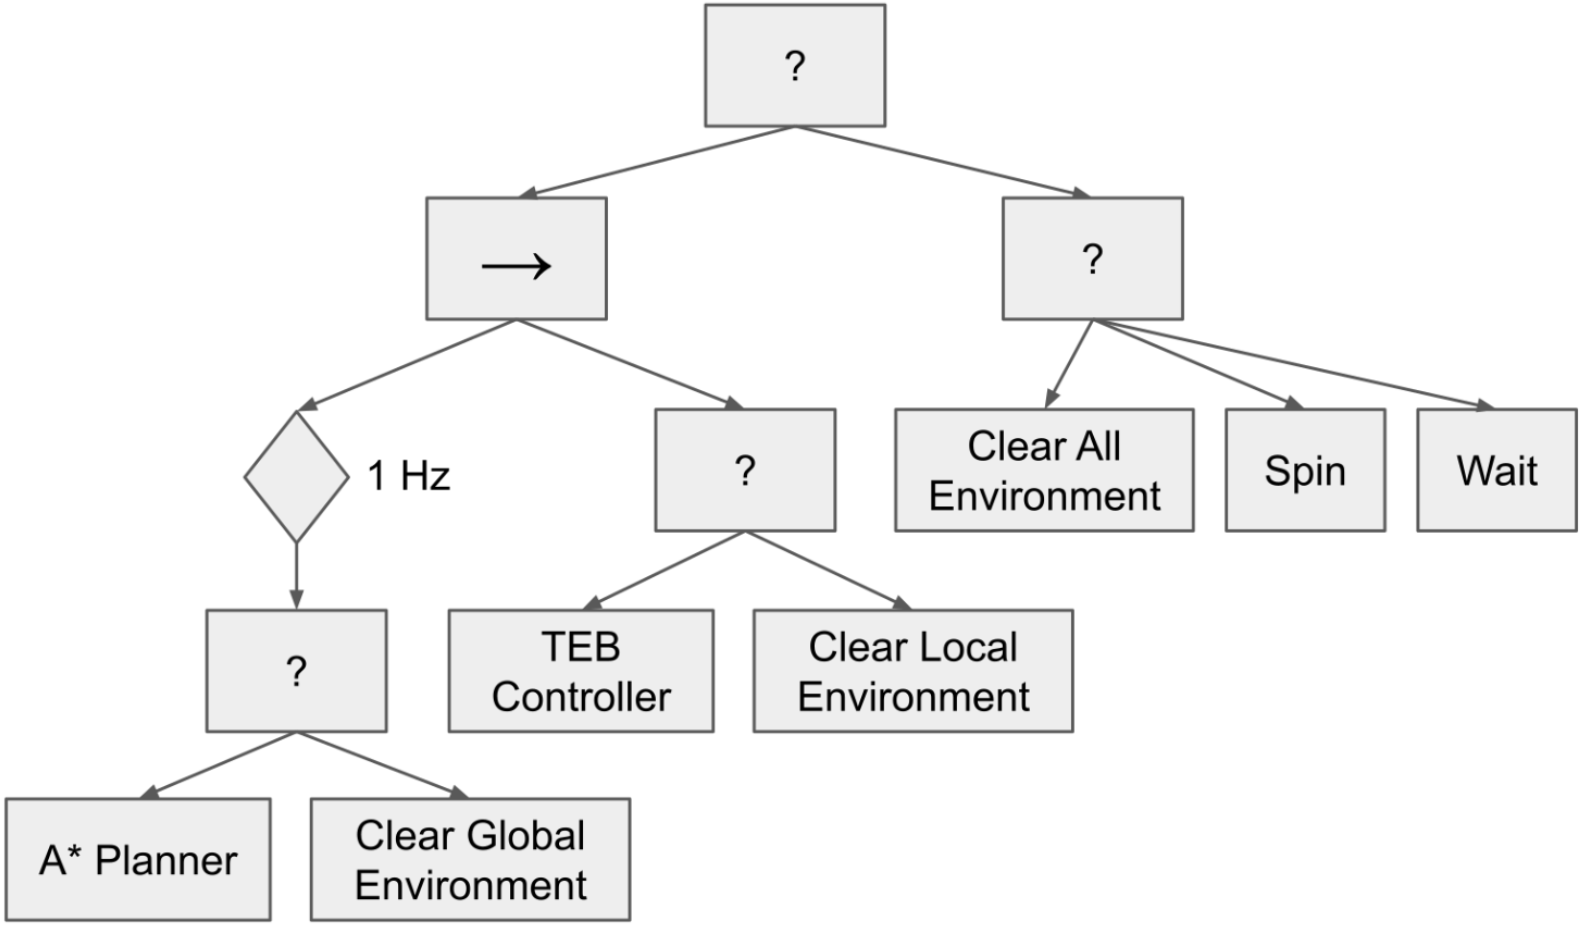
\includegraphics[width=\textwidth]{figures/20_state_of_the_art/nav2_bt.png}
    \caption[The default navigation behavior]{The default navigation behavior (Source: \cite{macenski_marathon_2020})}
    \label{fig:nav2_bt}
\end{figure}

\Glspl{bt} were developed for video games to describe the behavior of computer-controlled characters in a modular way \cite{hutchison_evolving_2010}. \Glspl{bt} combine a deliberative approach with reactive components. The internal structure of the tree establishes an overall plan of actions, ensuring goal-oriented behavior. However, reactive behavior can still be triggered through constant reevaluation of all conditions. 

A \gls{bt} consists of small building blocks that can be combined to create any control structure. The biggest difference from State Machines is that in \glspl{fsm}, a state-dependent transition is triggered after a specific input. In \glspl{bt}, on the other hand, the entire structure is updated at regular, short time intervals, and all conditions are re-evaluated. This allows for arbitrary transitions to occur based on the appropriate preconditions, without explicitly defining them.

The fundamental element of every \gls{bt} is the root node, from which the attached nodes are updated (ticked). Each node returns either Success, Failure, or Running after being updated. In general, a \gls{bt} can be described using an \gls{fsm}, where the state transitions can take three possible states into account, as shown in Figure \ref{fig:fsm_general_bt}.

\begin{figure}[h]
    \centering
    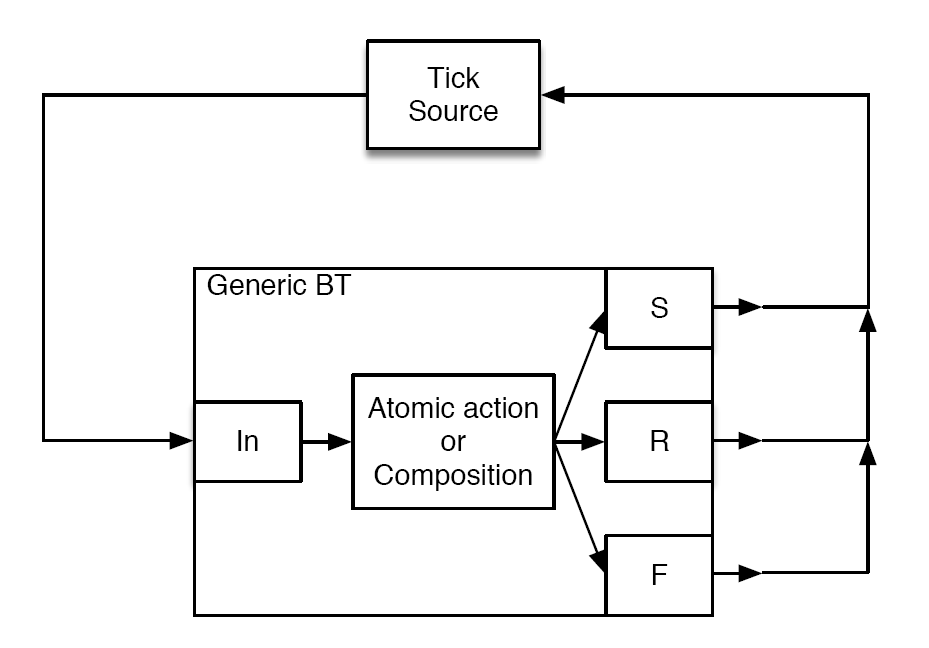
\includegraphics[width=0.7\textwidth]{figures/20_state_of_the_art/fsm_general_bt.png}
    \caption[General \gls{bt} displayed as \gls{fsm}]{General \gls{bt} displayed as \gls{fsm} with the state transitions: Success (S), Running (R) and Failure (F) (Source: \cite{colledanchise_behavior_2018})}
    \label{fig:fsm_general_bt}
\end{figure}

The basic building blocks of a \gls{bt} are shown in Figure \ref{fig:bt_types}. Actions represent individual, self-contained algorithms that execute specific commands to actuators or perform calculations. An Action can run in a blocking (synchronous) manner, where it returns either Success or Failure after its start, or it can run asynchronously and maintain a Running state during execution. Conditions, on the other hand, take either Success or Failure states depending on the condition being evaluated.

\begin{figure}[h]
    \centering
    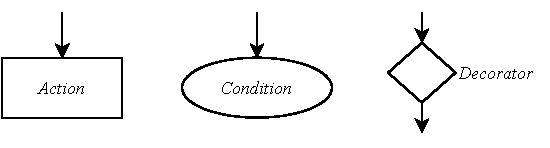
\includegraphics[width=0.7\textwidth]{figures/20_state_of_the_art/bt_types.pdf}
    \caption{Graphical representation of Actions, Conditions and Decorators}
    \label{fig:bt_types}
\end{figure}

The Decorator is a type of control node that has only one child. It allows the state of the child node to be influenced by custom-defined rules, avoiding complex constructions with Sequences and Fallbacks. Examples of Decorators include Inverters, Time Delays, and Repeaters (repeating a certain number of times or until a successful completion).

\begin{figure}[h]
    \centering
    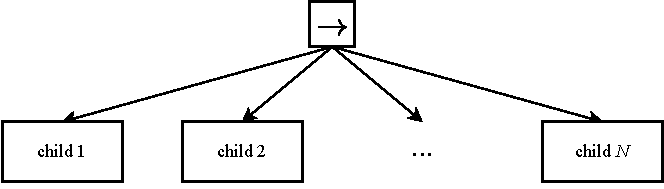
\includegraphics[width=0.75\textwidth]{figures/20_state_of_the_art/sequence.pdf}
    \caption{Graphical BT of a Sequence with \textit{N} childs}
    \label{fig:sequence}
\end{figure}

\lstset{language=C++, caption={Algorithm of a Sequence with \textit{N} childs}, label={lst:pseudo_code_sequence}, morekeywords={from, to}}
\begin{lstlisting}[float=h]
for i from 1 to %\textit{N}% do
    child_status = tick(child[i])
    
    if child_status == %\textit{Running}%
        return %\textit{Running}%
        
    if child_status == %\textit{Failure}%
        return %\textit{Failure}%

return %\textit{Success}%
\end{lstlisting}

The Sequence starts its children from left to right in the graphical representation, as shown in Figure \ref{fig:sequence}. If a child returns Running, the entire Sequence is considered Running. Upon successful execution of a child, the next child is started, continuing until all children, and thus the entire Sequence, achieve the Success state. If a child cannot be executed successfully, the loop is aborted, and the Sequence enters the Failure state, as shown in Algorithm \ref{lst:pseudo_code_sequence}.
  

\begin{figure}[h]
    \centering
    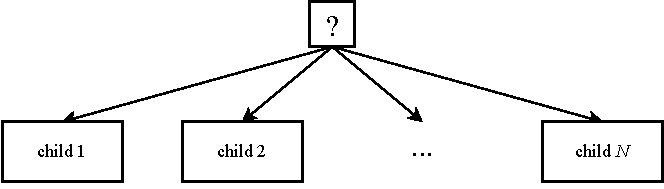
\includegraphics[width=0.75\textwidth]{figures/20_state_of_the_art/fallback.pdf}
    \caption{Graphical BT of a Fallback with \textit{N} childs}
    \label{fig:fallback}
  \end{figure}
  
  \lstset{language=C++, caption={Algorithm of a Fallback with \textit{N} childs}, label={lst:pseudo_code_fallback}, morekeywords={from, to}}
  \begin{lstlisting}[float=h]
  for i from 1 to %\textit{N}% do
      child_status = tick(child[i])
      
      if child_status == %\textit{Running}%
          return %\textit{Running}%
          
      if child_status == %\textit{Success}%
          return %\textit{Success}%
  
  return %\textit{Failure}%
  \end{lstlisting}

  A Fallback node (also known as Selector) executes only one child successfully, unlike the Sequence. All children are updated from left to right, as shown in Figure \ref{fig:fallback} and Algorithm \ref{lst:pseudo_code_fallback}. Once a child reaches the Success state, the Fallback is completed. If a child returns Failure, the next child is started.

\begin{figure}[h]
    \centering
    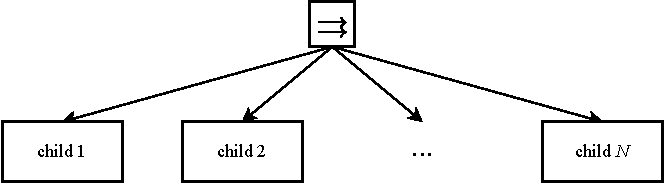
\includegraphics[width=0.75\textwidth]{figures/20_state_of_the_art/parallel.pdf}
    \caption{Graphical BT of a Parallel with \textit{N} childs}
    \label{fig:parallel}
\end{figure}
  
\lstset{language=C++, caption={Algorithm of a Parallel with \textit{N} childs and success count \textit{M}}, label={lst:pseudo_code_parallel}, morekeywords={from, to}}
\begin{lstlisting}[float=h]
for i from 1 to %\textit{N}% do
    child_status[i] = tick(child[i])
    
if success_count(child_status) >= %\textit{M}%
    return %\textit{Success}%
        
if failure_count(child_status) > (%\textit{N}% - %\textit{M}%)
    return %\textit{Failure}%

return %\textit{Running}%
\end{lstlisting}

In addition to the control nodes Sequence and Fallback, there is also the Parallel node. In this structure, all children are started simultaneously, and the final state of the Parallel node is determined based on a comparison between a defined count M and the number of successfully completed children, as shown in Figure \ref{fig:parallel} and Algorithm \ref{lst:pseudo_code_parallel}.

An overview of the functions of each element is presented in Table \ref{tab:overview_bt}.

\begin{table}[h]
\centering
\resizebox{\textwidth}{!}{%
%\setlength{\extrarowheight}{8pt}
\begin{tabular}{lclll}
\toprule
\textbf{} & \multicolumn{1}{l}{\textbf{}} & \multicolumn{3}{c}{\textbf{Return Status}} \\ \midrule
\multicolumn{1}{c}{\textbf{Type}} & \textbf{Symbol} & \multicolumn{1}{c}{\textbf{Success}} & \multicolumn{1}{c}{\textbf{Failure}} & \multicolumn{1}{c}{\textbf{Running}} \\ \midrule
\textbf{Action} & Text & When completed & In case of errors & During execution \vspace{3mm}\\
\textbf{Condition} & Text & When condition is true & When condition is false & Never \vspace{3mm}\\
\textbf{Sequence} & $\to$ & When all children are \textit{Success} & When a child is \textit{Failure} & When a child is \textit{Running} \vspace{3mm}\\
\textbf{Fallback} & ? & When a child is \textit{Success} & When all children are \textit{Failure} & When a child is \textit{Running} \vspace{3mm}\\
\textbf{Parallel} & $\rightrightarrows$ & \begin{tabular}[c]{@{}l@{}}When $\ge$ \textit{M} \\ children are \textit{Success}\end{tabular} & \begin{tabular}[c]{@{}l@{}}When > \textit{N} - \textit{M} \\ children are \textit{Failure}\end{tabular} & \begin{tabular}[c]{@{}l@{}}As long as limits \\ are not reached\end{tabular} \vspace{3mm}\\
\textbf{Decorator} & $\diamond$ & Depending on the function & Depending on the function & Depending on the function \\ \bottomrule
\end{tabular}%
}
\caption{Overview of the elements of a Behavior Tree}
\label{tab:overview_bt}
\end{table}

\Glspl{bt} represent an evolution of \gls{fsm}, which are still widely used, but offer several advantages beyond them. The following are the advantages and drawbacks of \glspl{bt}. These characteristics are not necessarily unique to \glspl{bt} but also apply to other concepts such as \glspl{hfsm} or decision trees \cite{colledanchise_behavior_2018}.

\begin{enumerate}
  \item \textbf{Modularity:} Individual subsystems can be modified and replaced as needed. The entire BT can also be reused as a module.
  \item \textbf{Hierarchical Structure:} Each control node introduces an additional level of hierarchy, making the overall behavior easier to understand.
  \item \textbf{Reusability:} Defined interfaces allow code to be used in multiple locations.
  \item \textbf{Reactiveness:} By continuously updating the BT, actions can be executed in a closed loop, enabling dynamic responses to the environment.
  \item \textbf{Intuitive Representation:} The graphical representation remains understandable even for complex systems.
  \item \textbf{Automatic Analysis:} Tools exist to monitor robustness and efficiency. BTs can also be created and monitored live using graphical editors.
  \item \textbf{Automatic Generation:} BTs can be generated during execution using machine learning techniques.
\end{enumerate}

However, there are also some disadvantages of BTs:

\begin{enumerate}
  \item \textbf{Complexity of the Engine:} Ensuring parallelism is necessary, but there are existing frameworks available to handle this.
  \item \textbf{Computational Intensity:} Updating all control nodes and conditions at each tick can be computationally intensive, potentially affecting real-time performance on weaker systems.
  \item \textbf{Implementation Overhead for Simple Behaviors:} For very short behaviors, direct programming or a simple FSM may be more efficient.
  \item \textbf{Immaturity of Behavior Trees:} Compared to widely adopted FSMs, there are fewer applications and software available for BTs.
\end{enumerate}


%% ==============================
\section{Hierarchical Path Planning}
\label{sec:hierarchical_planning}
%% ==============================

Other approaches to Q1 (Navigate in complex multi-floor environments):
\begin{enumerate}
    \item General Hierarchical Graphs (Latombe, Kavraki)
    \item Hierarchical D* algorithm with materialization of costs for robot path planning (Cagigas)
    \item Hierarchical path planning of mobile robots in complex indoor environments (Seder)
    \item Paper IAS-17 Autonomous Hierachy Creation for Path Planning of Mobile Robots in Large Environments
    \item Paper Hierarchical Path-Planning for Mobile Robots Using a Skeletonization-Informed Rapidly Exploring Random Tree*
    \item ROS1 Multi-floor example
    \item Amazon multi floor hospital (not found)
\end{enumerate}

This section presents the related work in the area of path planning with hierarchical graphs. This gives an overview of the relevant existing works corresponding to the first research question: "How to navigate in complex multi-floor environments?". 
A \Gls{h_graph} is a graph where each node in the graph holds a sub-graph itself. This is used for hierarchically structure information while the connections in on graph also represent information. The connections in a graph can be any configuration of non-directional, directional, bi-directional, sparse or densely connected. This depends on the data it stores. For navigation this data can be the logic separations of a complex environment like a research campus. The hierarchical layers could be buildings, floors, rooms and the gridmap itself. The structure of an \gls{h_graph} can be represented as a tree. An \gls{h_graph} with three hierarchical layers can be represented as a tree with a depth of three. An example of the structure of an \gls{h_graph} can be seen in Figure \ref{fig:h_graph}. The internal connections of the nodes in each graph is not represented in the figure. 

\begin{figure}[h]
    \centering
    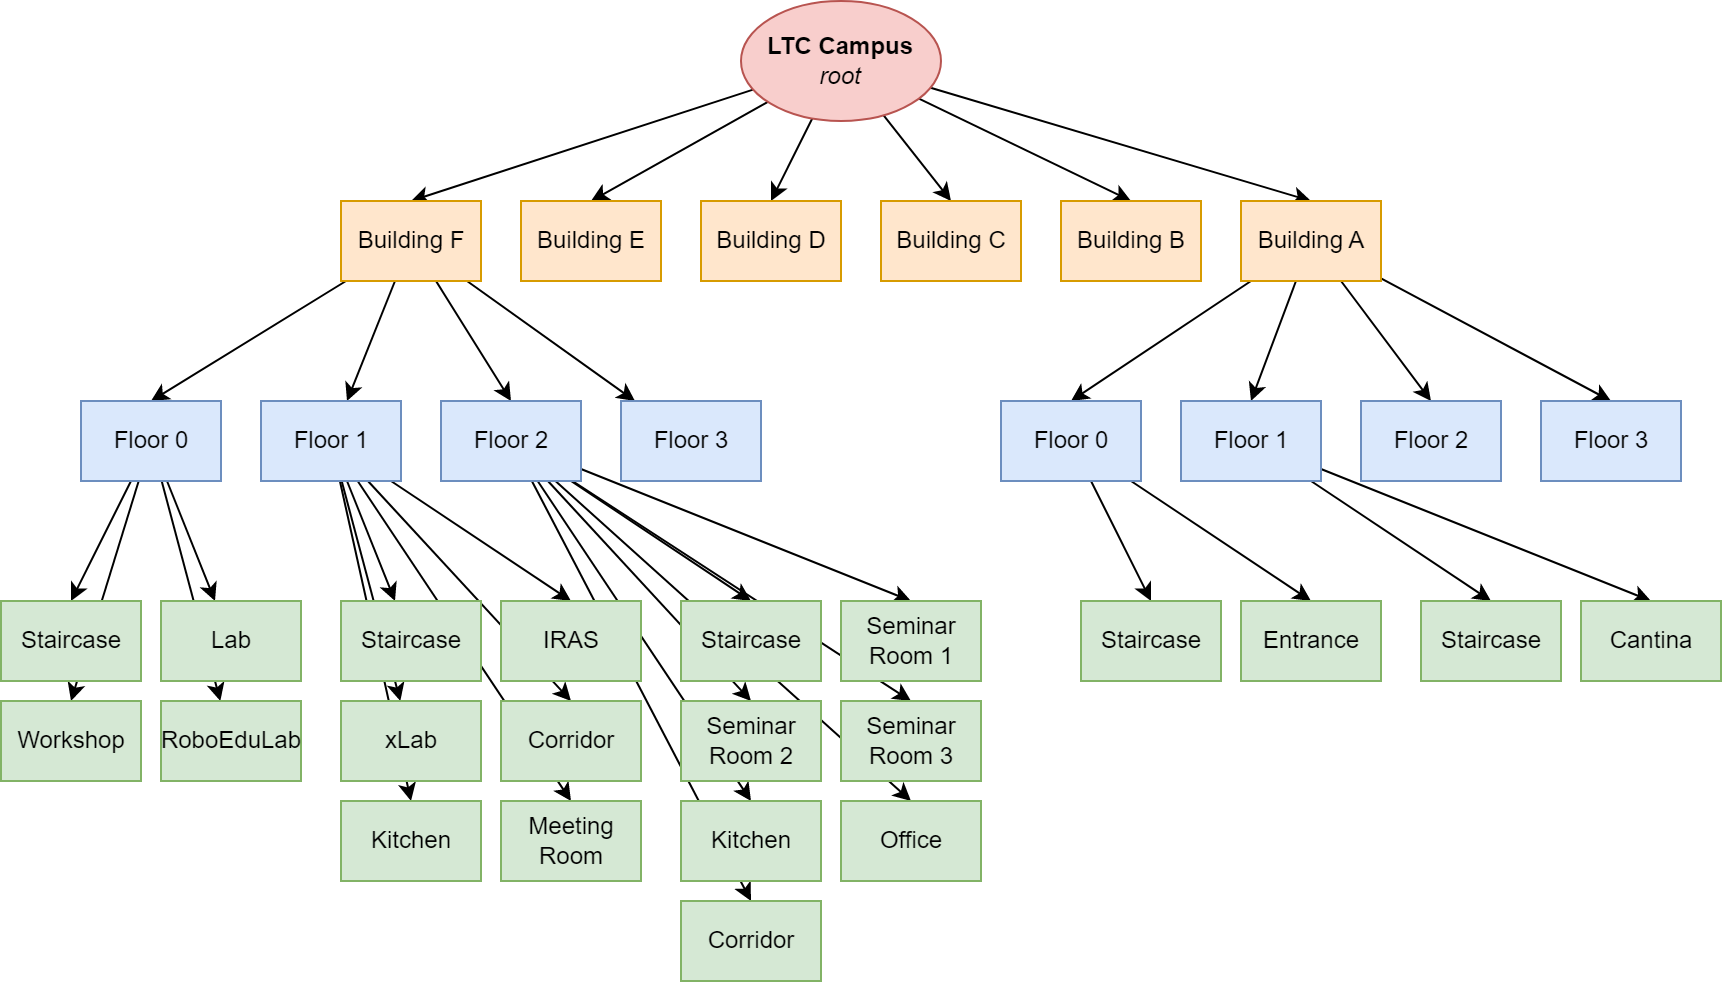
\includegraphics[width=\textwidth]{figures/20_state_of_the_art/hierarchical_graph.png}
    \caption[Representation of the structure of an H-Graph as tree]{Representation of the structure of an H-Graph with three hierarchical layers as a tree with depth of three. This example shows the whole campus on layer 0 (red), the buildings of this campus on layer 1 (orange), the floors of each building on layer 2 (blue) and the single rooms on layer 3 (green). For better visibility only some example nodes are fully expanded}
    \label{fig:h_graph}
\end{figure}

For use in navigation the structure of the \gls{h_graph} represents the physical environment, this was first applied to mobile robot path planning by \cite{fernandez_hierarchical_1998} \cite{fernandez-madrigal_multi-hierarchical_2001}. The nodes in each graph are connected only if a drivable connection between these buildings or rooms exits. To make this space plannable the connection has a cost corresponding to the shortest path distance between these two entities. This allows a common graph solver algorithm like Dijkstra or A* to find the shortest path in each graph. The advantage of a \gls{h_graph} is that not every leaf node in the tree has to be searched because only the nodes which are on the path of the higher layer are relevant. This reduces the search space and the time needed to find the optimal path in large environments drastically. To combine a feasible path from all different graphs on the lowest layer, continuity between paths of different subgraphs has to be ensured.

One proposed solution is the Hierarchical D* (HD*) algorithm from Cagigas \cite{cagigas_hierarchical_2005}. Cagigas breaks down an environment by hierarchical decomposition into an \gls{h_graph}. In each subgraph the shortest connections to elevators are precalculated and stored as weight of the connection in the meta-graph. This is called materialization of costs. After finding the shortest path based on these costs, a reconstruction process is applied that links the obtained partial paths. Cagigas extends the original D* algorithm \cite{hebert_optimal_1997} for this hierarchical planning. The D* algorithm is represents a dynamic or on-line version of the A* algorithm. The D* reuses and updates the calculated cost from the intial search to replan the path if an dynamic obstacle blocks the initial path. This is an efficient way to replan without calculating all costs again. Cagigas defines three types of hierarchical path planning: 
\begin{enumerate}
    \item \textbf{Horizontal path planning (HPP):} paths between nodes connected in a horizontal way. Equivalent to traditional robot path planning.
    \item \textbf{Vertical path planning (VPP):} paths between nodes connected in a vertical way. Namely, paths that begin on a floor and finish on another floor of the same building.
    \item \textbf{Inter-building path planning (IPP):} paths between nodes of different buildings. These paths begin on a floor of a building and finish on a floor of another building.
\end{enumerate}
Cagigas identifies the elevator selection problem shown in Figure \ref{fig:elevator_selection_problem} which occures in vertical path planning. The benefits of the HD* can not be applied here and a complete path replanning is necessary.

\begin{figure}[h]
    \centering
    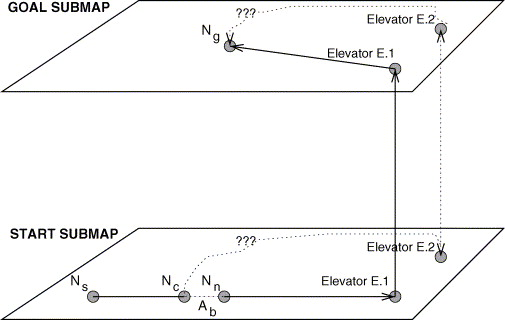
\includegraphics[width=0.75\textwidth]{figures/20_state_of_the_art/elevator_selection_problem.jpg}
    \caption[The elevator selection problem]{On-line vertical path planning. A “broken” arc \(A_b\) (obstacle) is detected between the current node \(N_c\) and the next node \(N_n\) in an initial path that joins a start node \(N_s\) and a goal node \(N_g\). The path planner module has to select an elevator entrance and there are two possibilities: the elevator entrance in the initial path (Elevator E.1) or an alternative elevator entrance (Elevator E.2). This last selection implies a complete path replanning. (Source: \cite{cagigas_hierarchical_2005})}
    \label{fig:elevator_selection_problem}
\end{figure}


In \cite{seder_hierarchical_2011} Seder proposed the Focussed Hierarchical D* (FHD*) algorithm. It improves the HD* algorithm by Cagigas in the following points:
\begin{enumerate}
    \item optimal placement of the so-called bridge nodes needed for hierarchy creation.
    \item focusing the search around the optimal path, which reduces the search area without loss of optimality.
    \item introduction of partial starts and partial goals, which further reduce computational time of replanning operations.
\end{enumerate}

Especially the optimal placement of bridge points is important to ensure optimal paths over multiple hierarchies. Bridge nodes are be placed at the optimal path that is to be followed by a mobile robot on its way from one room to the other. Seder calculates the optimal position by using a safety cost mask to find the middle point in a narrow passage. This corresponds to the safest point for a robot to drive through a door. In Figure \ref{fig:bridge_node_placement} an example of the bridge node placement can be seen. Seder shows, that the FHD* agorithm is faster during replanning, needs fewer iterations and fewer explored nodes compared to the D*, FD* and HD* algorithms.

\begin{figure}[h]
    \centering
    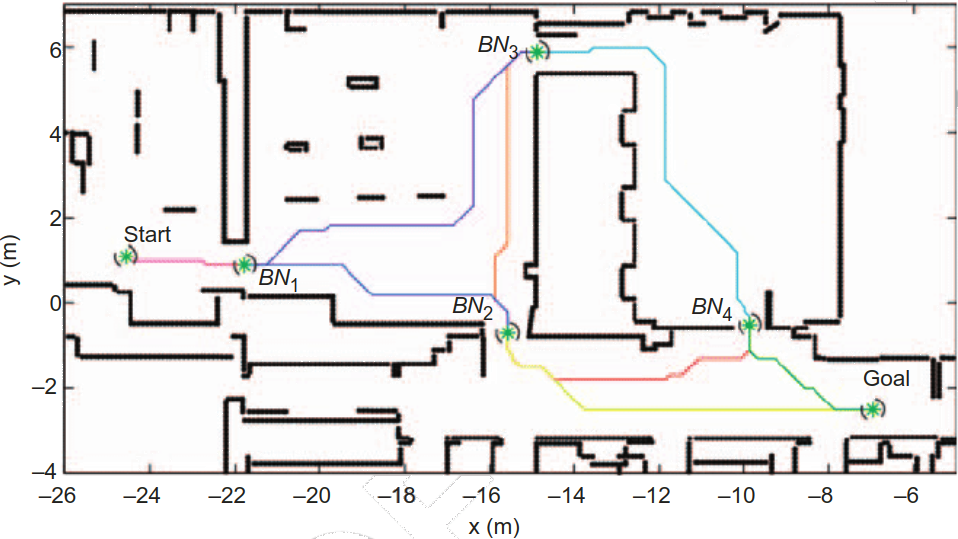
\includegraphics[width=0.75\textwidth]{figures/20_state_of_the_art/bridge_node_placement_paths.png}
    \caption[The bridge nodes with precalculated paths]{The bridge nodes BN 1-4 and the precalculated paths between them. (Source: \cite{seder_hierarchical_2011})}
    \label{fig:bridge_node_placement}
\end{figure}

Gregoric \cite{gregoric_autonomous_2022} further extends the ideas of Seder by using the E* algorithm \cite{philippsen_interpolated_2005}. This leverages the A* to plan with an arbitrary angle instead of a fixed grid with 90 degrees (4 neighbours) or 45 degrees (8 neighbours). Gregoric proposes a method to automatically generate an H-Graph from CAD floor plans. On floor map level this is done by using the safety cost mask. Connections between buildings are assumed to be on the ground floor. Vertical bridge connections are found with three conditions: 

\begin{enumerate}
    \item Comparing the positions of nodes on each floor
    \item The size of the room 
    \item The number of doors connecting this room to others
\end{enumerate}

Ryu uses a different approach in generation of the \gls{h_graph} as well as finding the subpaths \cite{ryu_hierarchical_2020}. Ryu only uses a two-layered hierarchy on a single floor. The two hierarchies are the so called inter- and intra-regional graphs which correspond to the connections between rooms and the path between the doors in each room. The hierarchy is automatically created by segmenting the entire floor plan into rooms. This is done by using the marker controlled watershed algorithm \cite{parvati_image_2009}. 

\begin{figure}[h]
    \centering
    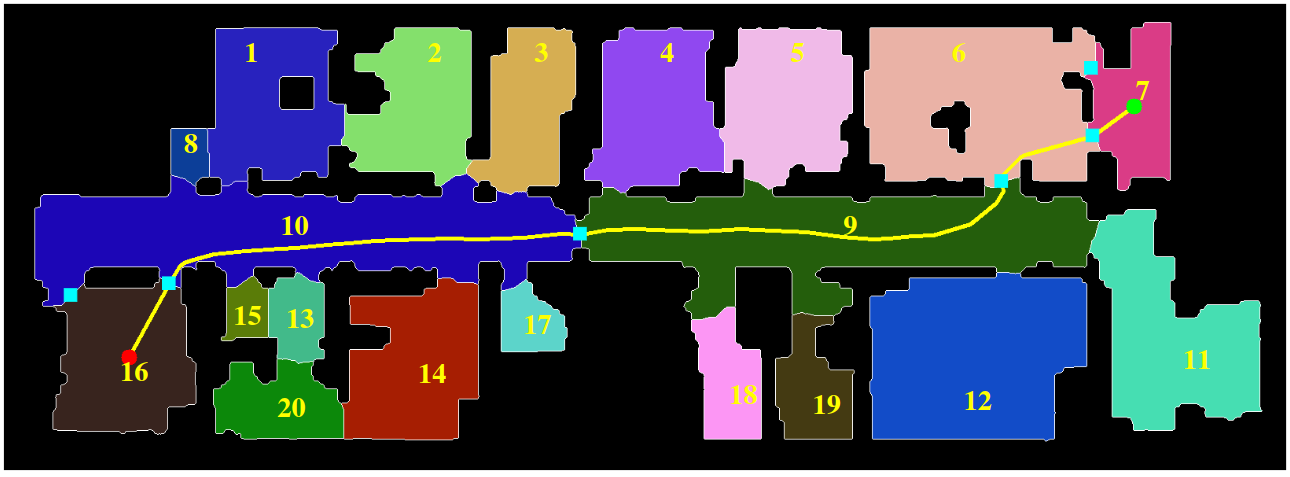
\includegraphics[width=0.75\textwidth]{figures/20_state_of_the_art/ryu_floor_path.png}
    \caption[The segmented floor map with combined inter-regional paths]{The segmented floor map with combined inter-regional paths (Source: \cite{ryu_hierarchical_2020})}
    \label{fig:ryu_floor_path}
\end{figure}

For the next step Ryu proposes an algorithm for detecting safe junction nodes as bridge between each room. A distance transform is used and the node with the highest clearance to the obstacle is chosen. This is similar to the process from Seder where a safety cost mask is applied. With these junction nodes the intra-graph is created as seen in Figure \ref{fig:ryu_floor_path}. Ryu then uses a Skeletonization-Informed Rapidly Exploring Random Tree* (SIRRT*) to plan the inter-regional path. This is an extension from the classic sample-based RRT algorithm. It uses a skeletonized representation of the grid map of a single room. This skeleton is used to inform the sampling of the RRT algorithm by generating nodes close to the skeleton. In Figure \ref{fig:ryu_sirrt} a solution path of the SIRRT* is shown. 

\begin{figure}[h]
    \centering
    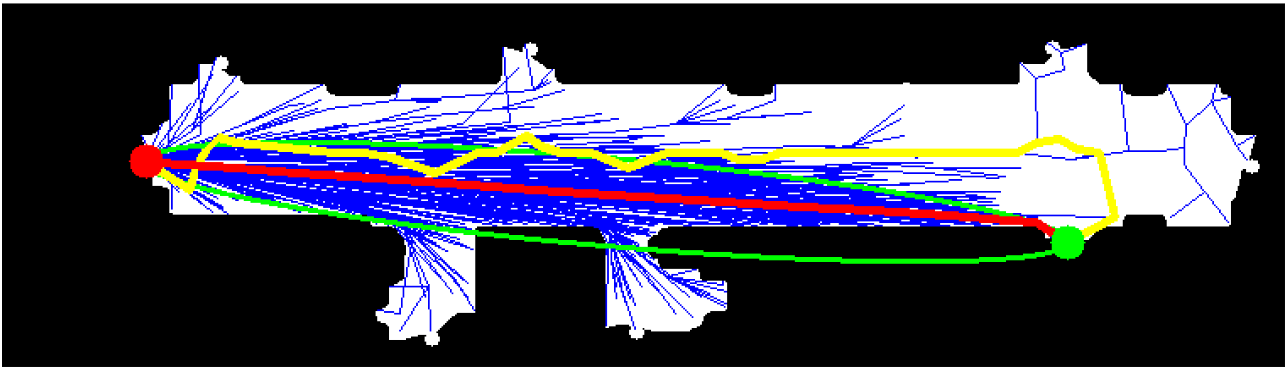
\includegraphics[width=0.75\textwidth]{figures/20_state_of_the_art/ryu_sirrt.png}
    \caption[Path planning with the SIRRT*]{An example of local path-planning for Segment “9” using the skeletonization informed rapidly exploring random tree* (SIRRT*): The red dot is the start position; the green dot is the goal. The initial skeleton path (yellow line). The final tree (blue line) and the optimized path (red line). The are for generating new sample nodes (green) (Source: \cite{ryu_hierarchical_2020})}
    \label{fig:ryu_sirrt}
\end{figure}

The previous papers were using simulated 2D gridmap environments. They have not mentioned the application on a real robot. Dihman et al \cite{dhiman_ros_2020} and Wang et al \cite{wang_autonomous_2019} separately introduced a framework for using multi-floor navigation with ROS 1 on a real robot. Wang uses a modified A* algorithm to plan paths that are more centered in the hallway. The main contribution is the development of an CNN to detect the current floor by pictures. A VGG16 network architecture is trained with 7,000 images to predict the current floor of the robot. It is not mentioned if automatic hierarchy creation or an H-Graph is used for navigation. It is also not mentioned how the robot knows which elevator or floors it needs to drive to. Only on floor map level path planning is done with the extended A*. Wang uses a real robot, the Pioneer 3-DX, and integrates everything in the existing ROS navigation stack. Dihman in comparison proposes a method for global path planning on a cost graph. This is one single graph to represent the floors and rooms of a single building, see Figure \ref{fig:dihman_cost_graph}. Vertical connections are drawn in the same graph and represented with corresponding traversal costs. Dihman also modifies the existing ROS 1 navigation stack to account for multiple robots and autonomous exploration. Additionally the map server is extended for a multi-level occupancy gridmap and the global planner plans with respect to the cost graph.

\begin{figure}[h]
    \centering
    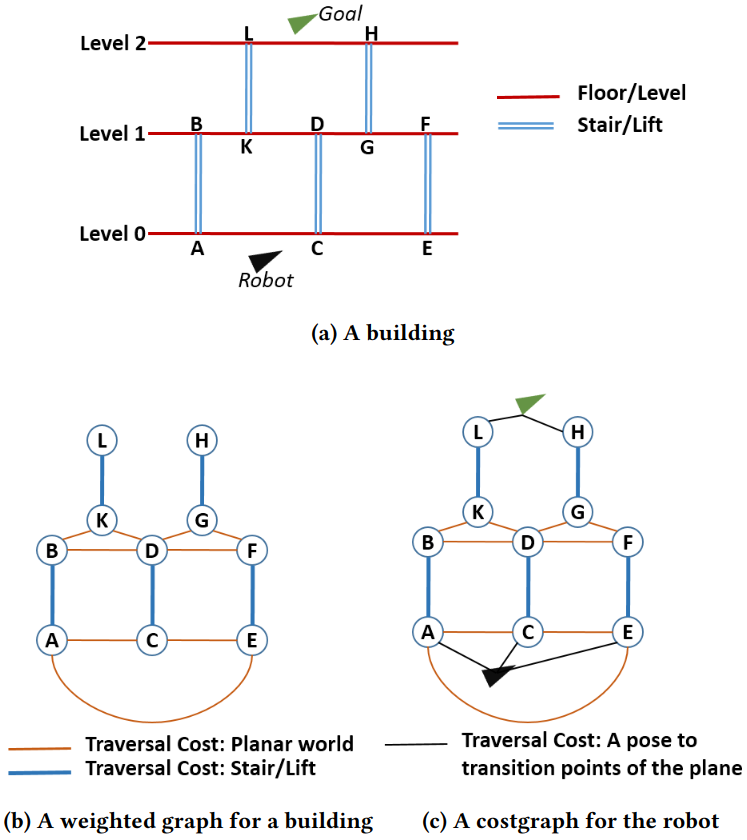
\includegraphics[width=0.75\textwidth]{figures/20_state_of_the_art/dihman_cost_graph.png}
    \caption[The costgraph for the robot]{(a) A building is represented as levels with stair or lift connection between floors, represented by thick blue parallel-lines. Blue and green color triangle represent current robot pose and goal pose respectively. (b) The building is transformed into a weighted graph. The node names refer to connection between the floor. (c) represents a weighted graph which includes edges from current robot pose and goal pose to the conncetion on the respective floor. This graph will be further used for solving global path planning. (Source: \cite{dhiman_ros_2020})}
    \label{fig:dihman_cost_graph}
\end{figure}

A comparison of these approaches to hierachical path planning in multi-floor environments is done in Chapter \ref{sec:research_gap}.
It can be seen, that the focus is either on the automatic hierarchy creation and efficient replanning or on the integration with ROS and the extension with additional features like CNN floor detection or multiple robots. This work aims to provide a mixture of these features by providing a method for automatic hierarchy creation for an H-Graph and integrating it in the new ROS 2 in simulation and for a real robot.

%% ==============================
\section{Straight Path Planning}
\label{sec:straight_paths}
%% ==============================

\begin{enumerate}
    \item Voronoi Diagrams, EVG (with sensory horizont)
    \item Smoothing algorithms (Bezier curves, B-Splines, Bechtold and Glavina, Latombe)
    \item ROS2 OpenRMF
    \item Paper Straight Skeleton Based Automatic Generation of Hierarchical Topological Map in Indoor Environment
    \item Semantic and Topological Mapping using Intersection Identification (Has comparison on the AWS hospital map!)
\end{enumerate}

In this section the recent approaches to straight path planning are presented. This gives an overview of the relevant existing works corresponding to the second research question: "How to plan paths that are straight, deterministic and human-predictable?"

A common approach in path planning is the creation of a roadmap. The advantages of roadmaps are that they are very efficient for replanning because the roadmap is not recalculated every time. Depending on the creation process roadmaps do not guarantee optimality but they provide a feasible answer within a short period of time. This is especially useful for motion planning in a higher dimension space for multi axis manipulators. The configuration space \(C\) in the case of plane 2D path planning has the same x and y axis as the real space. Obstacles in \(C\)-space are inflated by the size of the robot to find collision free paths.

\begin{displayquote}
    \enquote{The roadmap approach to path planning consists of capturing the connectivity of the robot's free space in a network of one-dimensional curves, called the roadmap, lying in the free space \(C_{free}\) or its closure \(cl(C_{free})\). Once a roadmap \(R\) has been constructed . it is used as a set of standardized paths. Path planning is thus reduced to connecting the initial and goal configurations to points in \(R\) and searching \(R\) for a path between these points. The constructed path, if any, is the concatenation of three subpaths: a subpath connecting the initial configuration to the roadmap, a subpath contained in the roadmap, and a subpath connecting the roadmap to the goal configuration.} \cite{latombe_robot_2003}
\end{displayquote}

In the previously presented RRT or PRM algorithm the roadmap is created by randomly sampling free points in \(C\)-space and connection them with a collision free egde. Another approach for roadmap creation is the Voronoi diagramm. The diagram is the set of all points with the largest distance to neighbouring obstacles. It consits of free paths which maximize the obstacle clearance.

\begin{figure}[h]
    \centering
    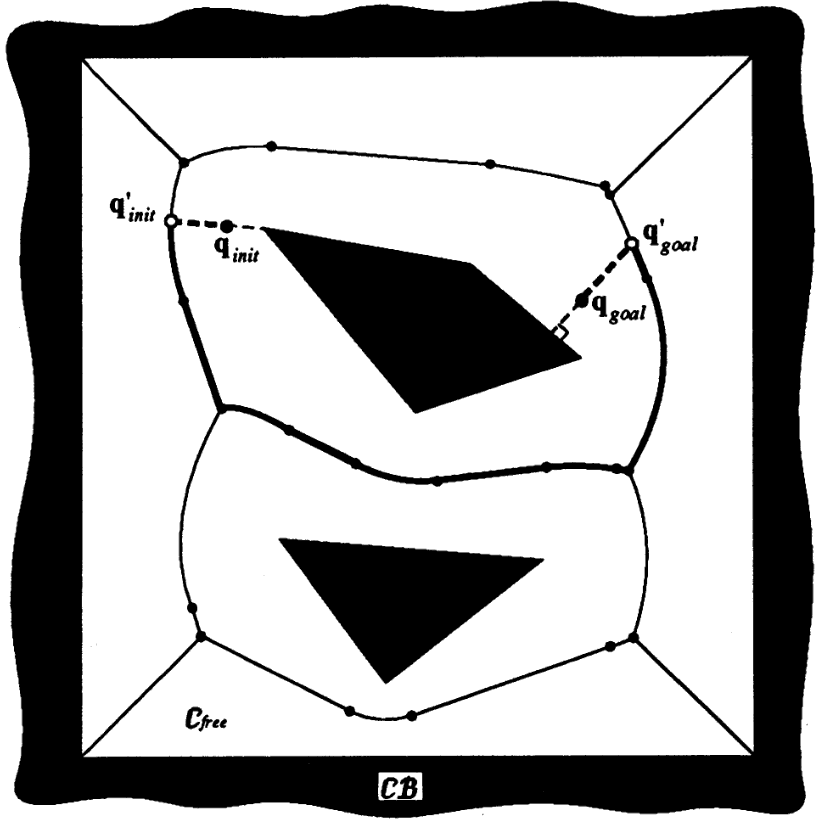
\includegraphics[width=0.5\textwidth]{figures/20_state_of_the_art/voronoi_diagram.png}
    \caption[The Voronoi diagram]{This figure shows the Voronoi diagram in a configuration space with a polygonal \(C\)-obstacle region. The free space is externally bounded by a rectangle. The initial and goal configurations \(q_{init}\) and \(q_{goal}\) are mapped into the Voronoi diagram to \(q'_{init}\) and \(q'_{goal}\), each by drawing the line along which its distance to the boundary to the \(C\)-obstacle region increases the fastest. (Source: \cite{latombe_robot_2003})}
    \label{fig:voronoi_diagram}
\end{figure}

The generalized Voronoi diagram, also called graph (GVG / GVD) is defined as the one-dimensional set of points equidistant to n or more obstacles in n-dimensions. By pruning the graph based on a minimum length the reduced generalized Voronoi graph (RGVG) can be obtained. Beeson et al. \cite{beeson_towards_2005} extended the GVD to solve a limited sensory horizont of mobile robots. The Extended Voronoi graph (EVG) transitions from a midleline in narrow corridors to a line which follows the walls in open rooms.  However the resulting paths suffer from noise in the measurements resulting in not straight paths. Also in junctions the GVD and EVG produce paths that bend into the intersections open space. Thus creating a unnecessary curve for the straight direction as seen in Figure \ref{fig:htm_path_comparison} c).

\begin{figure}[h]
    \centering
    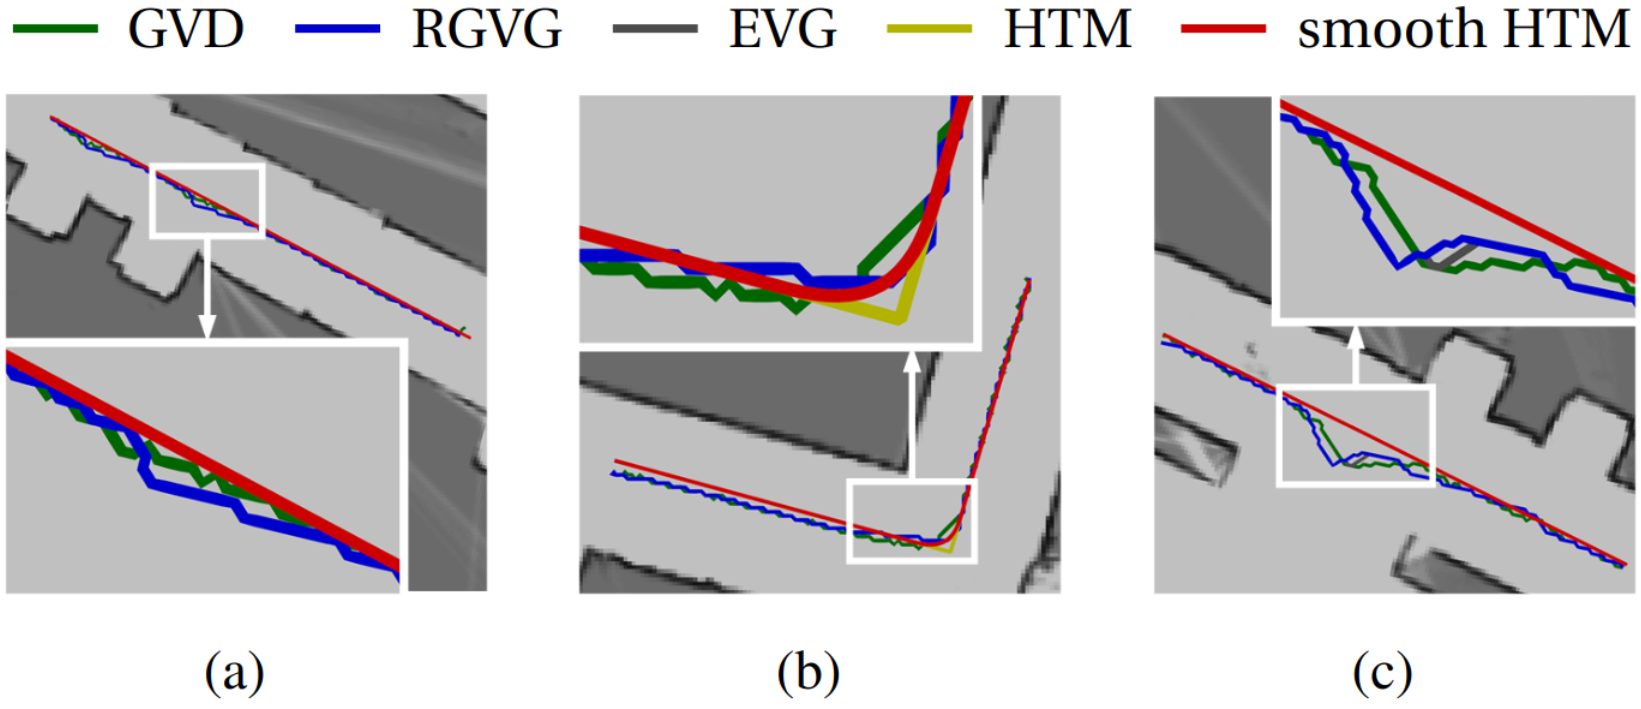
\includegraphics[width=0.75\textwidth]{figures/20_state_of_the_art/htm_path_comparison.png}
    \caption[Comparison between straight paths]{EVG based tracks coincide with RGVG based tracks within the sensory horizon. HTM based tracks coincide with smooth HTM when non-turning. (a) Tracks in the straight corridor. (b) Tracks in the turning corridor. (c) Tracks in the corridor with a room on the side. (Source: \cite{hou_straight_2021})}
    \label{fig:htm_path_comparison}
\end{figure}

Another approach for retrieving the topological map of an environment is the Straight Skeleton \cite{maurer_novel_1996}. In comparison to Voronoi diagrams this method does not use a distance function but shrinks the obstacle-polygon into the free space. Each edge is moved along its normal axis at the same speed, this creates a boundary where the shrinked edges touch. Based on this Straight Skeleton Hou et al. \cite{hou_straight_2021} improved the straight path generation and counters the jitter problem of the EVG. Hou et al. proposes the Hierarchical Topological Map (HTM) for the automatic generation of valid straight paths. The hierarchical approach first generates the straight skeleton and then detects intersections or small rooms where the jitter problem occures. These sections are extracted and a separate skeleton is generated inside which is then connected back to the global path. Finally a clothoid-based smoothing method is applied to ensure the curvature continuity of generated tracks. A comparison of the discussed algorithms for generating topological maps and straight paths can bee seen in Figure \ref{fig:htm_global_comparison}

\begin{figure}[h]
    \centering
    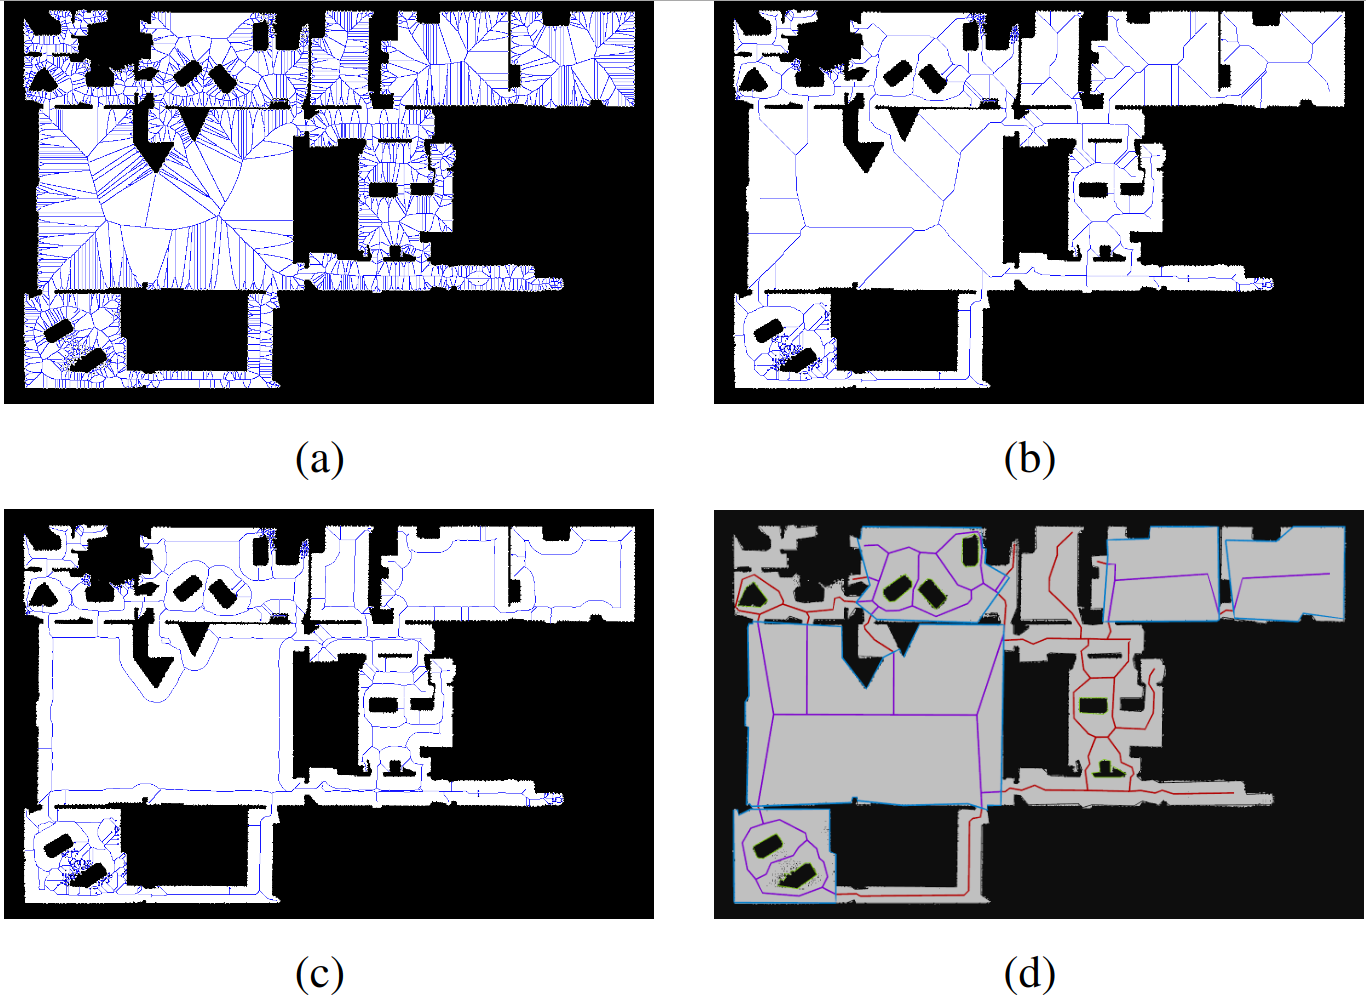
\includegraphics[width=\textwidth]{figures/20_state_of_the_art/htm_global_comparison.png}
    \caption[Comparison between straight paths]{Comparison of skeleton generation, using the grid map obtained from \cite{beeson_towards_2005}. (a) GVD. (b) RGVG. (c) EVG with a sensory horizon of 1.25m. (d) HTM. Primary tracks, secondary tracks, and regions are marked in red, purple, and blue, respectively. (Source: \cite{hou_straight_2021})}
    \label{fig:htm_global_comparison}
\end{figure}

The presented methods focus on the goal of extracting a topological map from the gridmap. The HTM also focuses on generating paths that a straight. Further discussion on the limitations of these approaches and the resulting research gap this work aims to address is done in Chapter \ref{sec:research_gap}. 

%% ==============================
\section{Research Gap and Limitations}
\label{sec:research_gap}
%% ==============================

Research gap from previous approaches:
\begin{enumerate}
    \item Hierarchical graphs are not per room or per floor which makes it difficult to append slamed maps or semantic information
    \item Hierarchical graphs are not used in ROS2 Nav Stack
    \item Approaches for straight paths are not deterministic and not human-predictable
    \item Approaches for straight paths are not implemented in ROS2 Nav Stack
    \item Approaches for straight paths only work well in small corridors
\end{enumerate}

Table with an overview of all related work
Author, algorithm, hierarchy levels, real robot, ROS1, ROS2, (automatic) hierarchy creation, Optimal, efficient replanning

Cagigas uses an environment with three hierarchy levels (floors, rooms and gridmap), no real robot or ROS, Manual hierarchy creation
Seder only uses a 2D floor-level environment with two hierarchies (rooms and gridmap), no real robot or ROS, automatic bridge point detection
Gregoric assumes a very simple multi-building environment where vertical bridge nodes are always directly above each other and connect only floors of the same building. Further buildings are assumed to have only one connection between each other on the ground floor. Although in complex environments bridges on upper floors, ramps or densely connected building sections are possible.
Ryu uses only a plane 2D environment on a single floor and creates a H-Graph with two hierarchy levels. This approach is not extended for a higher level of hierarchy. The Proposed SIRRT* is a fast algorithm but does not guarantee optimality. 
Wang implements a floor detection with CNN wich can be counted as a kind of hierarchy creation. But multi-floor planning is not discussed. Wang implements his work on a real robot with ROS 1.
Dihman uses a different approach with a single weighted graph for hierarchy representation. It is not created automatically but he uses multiple robots ans exploration to obtain the gridmaps. This is also implemented on ROS 1.

The HTM also focuses on generating paths that a straight. This makes these paths predictable for humans walking in the same area as the mobile robot. Also all of these approaches are deterministic. This means, given the same gridmap, these algorithms always produce the same output path. There is not a probabilistic function involved which generates random points like in the RRT or PRM. A path that is deterministic is also more predictable for humans as the robot behaves the same. The advantage is that humans working in the same space can learn the paths of the mobile robot and can predict areas where a robot might drive through. This is useful for the hospital environment of the PeTRA use-case. However the generated paths or not ideal for open spaces and large rooms as seen in Figure \ref{fig:htm_global_comparison} d). Assuming this is a lobby or other large room where people might wait and walk between doors. The path generated by the HTM are not intuitive. One would expect a robot to drive in a straight path parallel to the wall and not in a triangle shape driving at an angle and then returning to the same wall again. 
%% ==============================
\chapter{Methods}
\label{sec:methods}
%% ==============================
The general methodology of this work follows an iterative design principle. First, related work with specific approaches was analyzed. These approaches used benchmark environments to test their implementation and compare it to previous approaches. These benchmarks were used as a starting point for the development of the planner for this work. In the first evaluation phase, the developed planner was compared to other algorithms on the same benchmarks. A new metric was developed to quantify the disturbance of the public space. In the next step, the hierarchical planner was tested on a model of a real building. To combine these concepts, they were integrated into the \gls{nav_2} stack and tested in a simulated hospital environment. Throughout these steps, the code was continuously improved and debugged.

A limitation of the methodology of his work is that no comparative evaluation of the developed hierarchical planner with related work has been performed. This is due to the fact that the focus of this work is the implementation on a real robot with ROS 2, unlike older approaches that used different frameworks and did not publish the code online as open source. Also, the optimization of the developed planner in terms of computational speed was not the scope of this work. As a result, direct comparisons of planning times and other metrics of the hierarchical planner are lacking. A comparison of the straight path planner was performed as described in the following sections.

%% ==============================
\section{Existing Benchmarks}
\label{sec:benchmarks}
%% ==============================
 As seen in the literature review in Chapter \ref{sec:state_of_the_art}, most related works used common benchmarks to test their approaches. Specifically, the benchmark from \cite{ryu_hierarchical_2020} was used to test hierarchy creation and two-level hierarchical planning. This environment is a map of a real building. It was originally recorded by Stachniss \cite{cyrill_stachniss_robotics_2015} on the campus of the University of Freiburg, see Figure \ref{fig:freiburg_benchmark}. The second benchmark environment was previously shown in Figure \ref{fig:htm_global_comparison} and is mainly used to compare the straight path planner with the previous approaches. It was also used by Hou et al. \cite{hou_straight_2021} with the SIRRT* planner and by Beeson et al. \cite{beeson_towards_2005} with the EVG planner.

\begin{figure}[h]
    \centering
    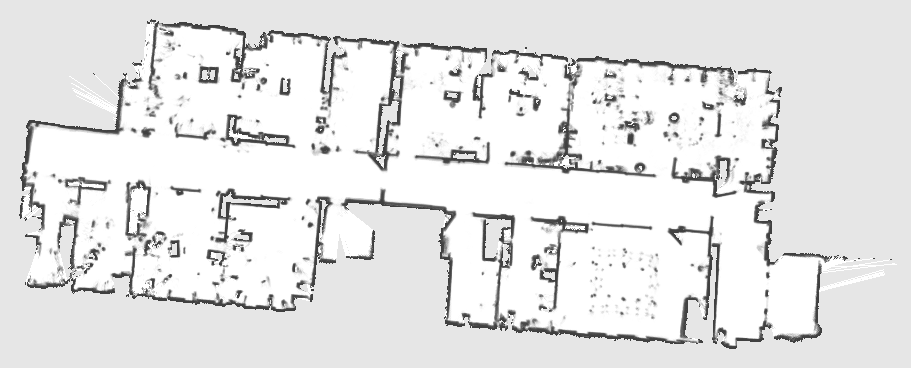
\includegraphics[width=0.75\textwidth]{figures/30_methods/freiburg_benchmark.png}
    \caption[The benchmark environment for hierarchy creation and straight path planning]{The benchmark environment for hierarchy creation and straight path planning recorded in the University of Freiburg (Source: \cite{cyrill_stachniss_robotics_2015})}
    \label{fig:freiburg_benchmark}
\end{figure}

In the first evaluation phase of the iterative process, the developed straight path planner is tested on these benchmark environments and compared to related work and common path planner algorithms. To ensure reliable and statistically significant results, each planner is tested on different benchmarks and the corresponding submaps of a single room. Each planner produces a number of paths resulting from the number of combinations of start and goal positions. These positions consist of \(n_r\) randomly sampled points in the drivable area and all bridge points \(n_b\) of the environment or submap. The total number of paths \(n_{\text{paths}}\) results from selecting two of these points from the start and goal points and repeating this for all possible combinations. This can be expressed by the binomial coefficient formula, where \(k\) is 2 because there is only one start point and one goal point, see the Equation \ref{equ:binomial_coefficient}.
\begin{equation} \label{equ:binomial_coefficient}
    n_{\text{paths}} = \binom{n_r + n_b}{2} = \frac{(n_r + n_b)!}{2! ((n_r + n_b)-2)!}
\end{equation}
In the case of one example room, there are 3 bridge points \(n_b\) and an additional 10 random points \(n_r\), resulting in 78 paths. In the case of the complete floor from the benchmark in Figure \ref{fig:freiburg_benchmark} \(n_b = 27\) and \(n_r = 20\), resulting in 1081 paths. These paths were then evaluated using the following metrics:
\begin{enumerate}
    \item \textbf{Success Rate}: Percentage of valid paths found
    \item \textbf{Path Length}: Total length from start to goal in pixels
    \item \textbf{Planning Time}: Total planning time including smoothing
    \item \textbf{Path Smoothness}: Sum of deviation angles divided by path length
    \item \textbf{Obstacle Clearance}: Mean distance from path to obstacles
    \item \textbf{Distance Deviation}: Standard deviation of distance between path and obstacles
    \item \textbf{Distance to Centroid}: Mean distance of the path to the centroid of the room
    \item \textbf{Disturbance of Public Space}: Largest open area within the map divided by total room area (details in Chapter \ref{sec:new_metric})
\end{enumerate}

%% ==============================
\section{New Metric for Disturbance of Public Space}
\label{sec:new_metric}
%% ==============================
The problem statement in Chapter \ref{sec:problem_statement} presents the need for straight, deterministic, and predictable paths. In certain situations, it is important to drive close to the walls and not directly across the room. Such a scenario is shown in Figure \ref{fig:straight_path_problem}. In order to measure the planner's ability to produce paths that by design have little impact on the public space, a new metric must be invented. So far, there is no such metric in the literature because most path planning problems focus on finding the shortest possible solution. In contrast, this work focuses on straight paths and predictability. To avoid driving directly through a major human traffic route or through the queue of an information desk, this planner tries to stay close and parallel to the walls. This new metric provides a way to quantify this behavior. Unlike most path metrics and all of the metrics mentioned in the previous chapter, this new metric cannot be calculated from a single solution path. It gives a value for how well all possible paths in the map combined avoid the public space. The process of obtaining this value for one single room is described in the following:

\begin{enumerate}
    \item Get all bridge points \(n_b\) connecting this room to neighboring rooms or other hierarchies.
\item Sample \(n_r\) random points within the valid area (default \(n_r = 10\))
    \item Plan paths for all possible connections given by the equation \ref{equ:binomial_coefficient}
    \item Overlay all paths on the original room environment \(R\)
    \item Segment the room into connected components \(CC_{\text{free}}\) that are not separated by paths
    \item Get the largest connected components by area \(CC_{\text{free, max}} = \max \{\text{area}(CC_{\text{free}})\}\)
    \item Divide by the total area of the room and subtract from 1 to get the disturbance value \(D\) as in the equation \ref{equ:disturbance}.
\end{enumerate}
\begin{equation}
\label{equ:disturbance}
    D = 1 - \frac{\max \{\text{{area}}(CC_{\text{{free}}})\}}{{\text{{area}}(R)}}
\end{equation}

This results in a metric measuring public space disturbance for a single room, where a low value indicates desirable behavior for a mobile robot. Figure \ref{fig:disturbance_example} shows a comparison of the metric on a room from the second benchmark.

\begin{figure}[h]
    \captionsetup[subfigure]{justification=centering}
    \centering
    \begin{subfigure}{.5\textwidth}
      \centering
      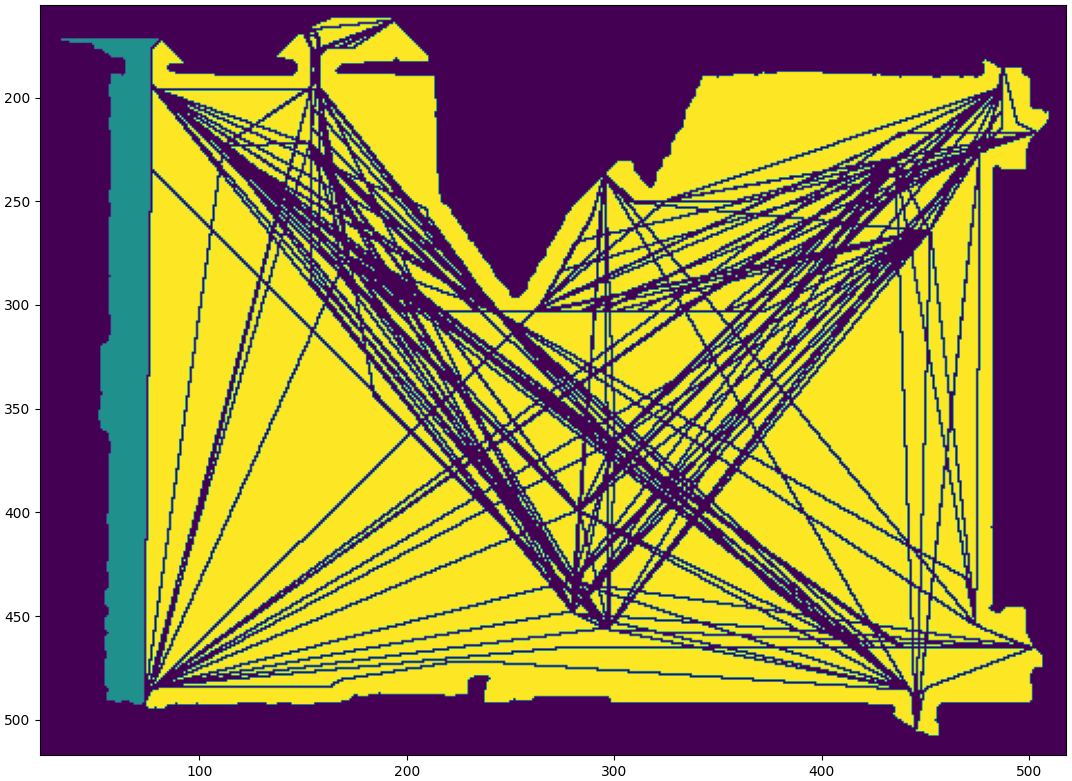
\includegraphics[width=\textwidth]{figures/30_methods/room9_disturbance_astar_smooth.png}
      \caption{Planner: A*, \(D = 0.95\)}
    \end{subfigure}%
    \begin{subfigure}{.5\textwidth}
      \centering
      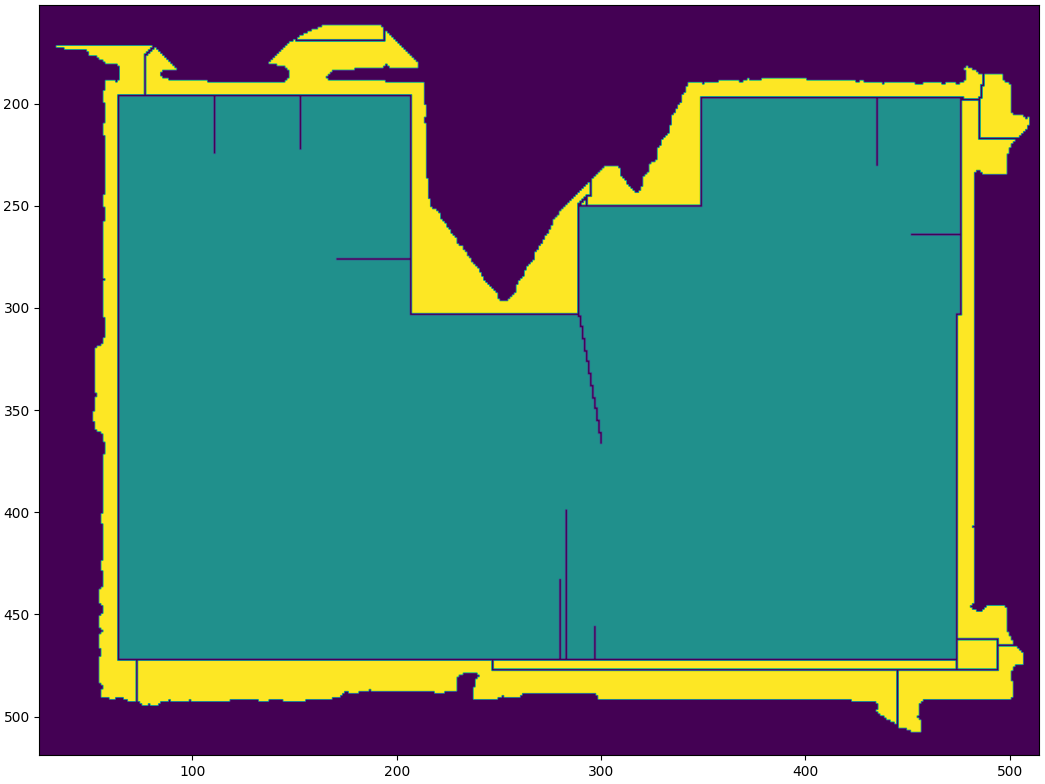
\includegraphics[width=.975\textwidth]{figures/30_methods/room9_disturbance_ilir_smooth.png}
      \caption{Planner: ILIR, \(D = 0.20\)}
    \end{subfigure}
    \caption[Example of the metric for disturbance of public space]{Example of the metric for the disturbance of public space with \(n_r=10\), \(n_b=9\), \(n_{\text{paths}}=171\). The area of the original room \(R\) in yellow and turquoise, the paths and walls in purple and the largest free area \(CC_{\text{free, max}}\) in turquoise.}
    \label{fig:disturbance_example}
\end{figure}

%% ==============================
\section{Simulation}
\label{sec:simulation}
%% ==============================
After developing hierarchy generation and two-level hierarchical planning, a more complex environment was needed to evaluate hierarchical planning with arbitrary hierarchical levels and connections between them. For this purpose, the campus of our research lab was modeled as a graph and used for planning. This environment is complex in terms of hierarchical connections, e.g. some stairs connect the second floor diagonally to the terrace of the first floor, which itself is shaped in a ring connecting all other buildings. This makes this environment more complex than a simple building with a vertical connection through an elevator, as used in previous work such as Gregoric et al. \cite{gregoric_autonomous_2022} or Cagigas \cite{cagigas_hierarchical_2005}. An image of the campus and the corresponding graph can be seen in Figure \ref{fig:ltc_rendering}.

\begin{figure}[h]
    \captionsetup[subfigure]{justification=centering}
    \centering
    \begin{subfigure}{.5\textwidth}
      \centering
      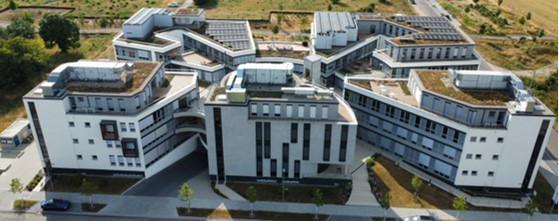
\includegraphics[width=\textwidth]{figures/30_methods/ltc_real.jpg}
      \caption{\gls{iras} campus}
    \end{subfigure}%
    \begin{subfigure}{.5\textwidth}
      \centering
      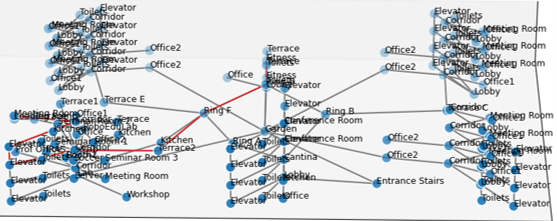
\includegraphics[width=\textwidth]{figures/30_methods/ltc_graph.png}
      \caption{Graph representation}
    \end{subfigure}
    \captionsetup{justification=centering}
    \caption[Image and graph representation of the \gls{iras} research campus]{Image a) and graph representation b) of the \gls{iras} research campus.}
    \label{fig:ltc_rendering}
\end{figure}

Both concepts, the hierarchical planner and the straight path planner, were combined and integrated into the \gls{nav_2} stack for \gls{ros_2}. For quick testing, this was done in a simulated hospital environment. This helps with debugging and accelerates development. The publicly available "AWS RoboMaker Hospital World" from Amazon \cite{aws_robotics_aws_2023} was used. Figure \ref{fig:aws_hospital} shows the simulated hospital. The advantage of this environment is that it also provides models for two and three floors. From this simulation the gap to the real world is small and it can finally be implemented on the real PeTRA robot.

\begin{figure}[h]
    \centering
    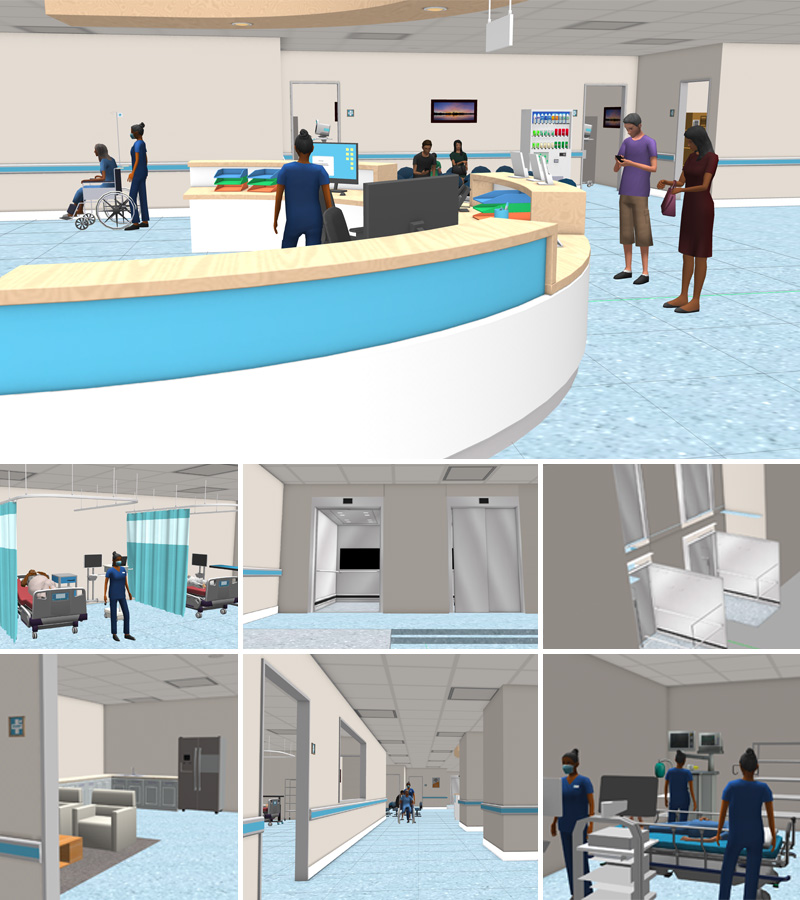
\includegraphics[width=0.5\textwidth]{figures/30_methods/hospital_world.jpg}
    \caption[The "AWS RoboMaker Hospital World" simulation environment for Gazebo]{The "AWS RoboMaker Hospital World" simulation environment for Gazebo. (Source: \cite{aws_robotics_aws_2023})}
    \label{fig:aws_hospital}
\end{figure}
%% ==============================
\chapter{Concept}
\label{sec:concept}
%% ==============================
Questions to ask:
\begin{enumerate}
    \item What is the high level concept of your work?
    \item What are important design decisions?
    \item Why did you choose this concept and what are the alternatives?
    \item What are drawbacks of your concept?
    \item How does your concept exceed existing approaches?
    \item How does this concept solve your research question?
\end{enumerate}

\begin{enumerate}
    \item Creation of semantic hierarchical graphs
    \item Algorithms with Pseudocode
    \item Usage of semantic informations
    \item Speed zones, no-go zones special locations
\end{enumerate}
%% ==============================
\chapter{Implementation}
\label{sec:implementation}
%% ==============================
Questions to ask:
\begin{enumerate}
    \item Which frameworks from others do you use? (open source tools)
    \item Which algorithms do you use?
    \item Which programming language do you use and why did you choose it?
    \item What code patterns did you apply?
    \item How does the most relevant part of your code work? (Pseudocode?)
    \item Which parameters can be used for configuration?
    \item How did you find the used set of parameters?   
    \item What are the interfaces for the end user?
    \item How to use your work?
\end{enumerate}

What is the software or hardware system used to implement the research ideas? 

Which frameworks or approaches from previous work are used? 

What are the main design choices and trade-offs in your system? 

What are the main implementation challenges and solutions? 

(If relevant) Which algorithms are used? (With pseudocode) 

\begin{enumerate}
    \item Algorithms LIR, OpenCV, Watershed
    \item Structure of semantic hierarchical graphs
    \item ROS2 Nav stack
    \item Implementation on the real PeTRA Robot
    \item Operating a real elevator 
\end{enumerate}

The planner is implemented as a plugin for the \gls{ros_2} and is evaluated using realistic simulation scenarios and real-world experiments. The planner is designed to be modular and can be easily integrated with the existing navigation stack. The planner is also designed to be scalable and can be used in environments of varying sizes and complexity.

Python is used and libraries numpy, opencv, shaply

%% ==============================
\section{Hierarchy Creation}
\label{sec:hierarchy_creation}
%% ==============================

The input for hierarchy creation is the raw occupancy gridmap from the SLAMing process of the robot. For the evaluation and better comparison the same benchmark map as used for the algorithm from \cite{ryu_hierarchical_2020} is taken. For better readability the image of this raw occupancy gridmap from Chapter \ref{sec:benchmarks} is shown again here in Figure \ref{fig:freiburg_benchmark_2}.

\begin{figure}[h]
    \centering
    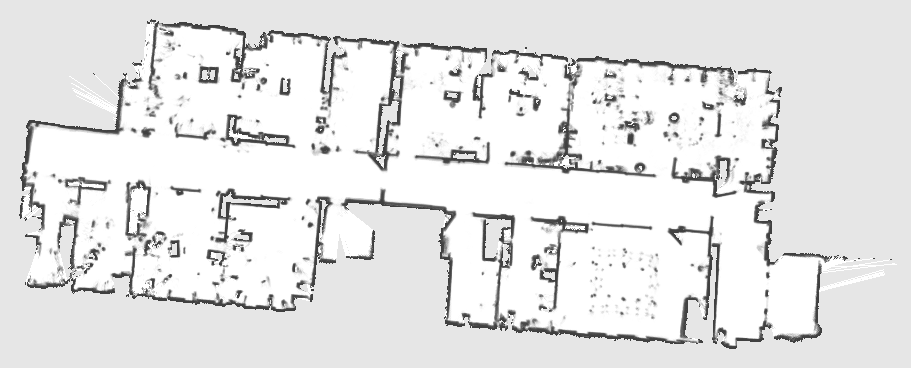
\includegraphics[width=0.75\textwidth]{figures/30_methods/freiburg_benchmark.png}
    \caption[The benchmark environment for hierarchy creation and straight path planning (intentional repetition)]{The benchmark environment for hierarchy creation and straight path planning recorded in the University of Freiburg (Source: \cite{cyrill_stachniss_robotics_2015})(intentional repetition)}
    \label{fig:freiburg_benchmark_2}
\end{figure}

This gridmap is build with the laser scanners of the mobile robot starting from the current pose at the time of starting the mapping. This starting pose is often not aligned with surrounding walls resulting in an apparent angle between the walls and the coordinate frame of the gridmap. This is not a problem for localization or path planning but makes it difficult to plan straight paths parallel to the walls. To solve this problem a rotation detection and outlier reduction algorithm is used.

\begin{figure}[h]
    \centering
    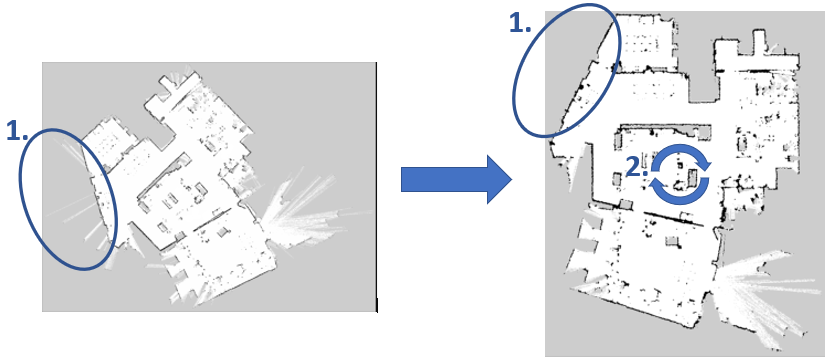
\includegraphics[width=0.75\textwidth]{figures/50_implementation/model_preprocessing_goal.png}
    \caption[Map preprocessing with rotation and outlier detection]{Map preprocessing with rotation and outlier detection. Original map on the left with outliers caused by transparent windows (1.). Resulting map on the right, outliers removed (1.) and rotation aligned with wall directions (2.) (Source: Tim Albert)}
    \label{fig:map_preprocessing}
\end{figure}

In Figure \ref{fig:map_preprocessing} the result of the preprocessing algorithm is seen. The algorithm first performs dilation and detects connected components. Based on the size these components are classified as outliers and the corresponding walls and white trails (see Figure \ref{fig:map_preprocessing} 1.) are removed. Then with the Probabilistic Hough Transform \cite{matas_robust_2000} straight lines are detected which represent the walls of the rooms. Finally the main orientation based on the most wall lines going in the same direction is chosen. To account for walls of one room and the adjacent wall perpendicular to it, the detected lines are clustered with the \gls{dbscan} algorithm \cite{ester_density-based_1996}. After obtaining the major rotation angle of the walls, the whole map is rotated to align with the coordinate frame of the gridmap. As this was developed and tested in an independent project it is not in the scope of this work.

The resulting map is now rotated parallel to the walls and outliers are removed. However there are still some artifacts in the map which obscure the real shape of the room. For best results some manual cleaning is still necessary. Most of these objects are dynamic obstacles which were at these positions during the mapping process but could be moved somewhere else by now. To not depend on this current snapshot of the environment the real shape of the room is estimated. The obstacles are later considered during the actual driving process. The task of the controller is to avoid these obstacles and provide a path around it. If this is not possible within the limits of the controller a replan is triggered. The resulting cleaned map is then binarized with a threshold and can bee seen in Figure \ref{fig:map_cleaned}

\begin{figure}[h]
    \centering
    
\includegraphics[width=0.75\textwidth]{figures/50_implementation/ryu.png}
    \caption[Binary map after rotation and manual cleaning]{Binary map after rotation and manual cleaning}
    \label{fig:map_cleaned}
\end{figure}

The segmentation of this map into single rooms and corridors is now done with the marker-controlled watershed algorithm \cite{parvati_image_2009}. For this the gridmap is converted into an numpy matrix and processed with opencv. OpenCV offers implementations for common image processing operations in python with which the watershed representation can be created. The process starts creating markers with which the normal watershed algorithm can be improved. Without predefined markers, watershed results in an over segmentation. For this an distance transform is performed on the image from Figure \ref{fig:map_cleaned}. This creates a mapping of each white pixels distance to the nearest black pixel. This can be interpreted as the obstacle clearance of this position and corresponds to the safety cost mask from Seder \cite{seder_hierarchical_2011}. By thresholding this distance map on a reasonable distance value d, the resulting binary image shows in white all pixels that have a distance greater or equal to d as seen in Figure \ref{fig:distance_transform}. Thus it represents the areas where most likely rooms are located. 

\begin{figure}[h]
    \captionsetup[subfigure]{justification=centering}
    \centering
    \begin{subfigure}{.5\textwidth}
      \centering
      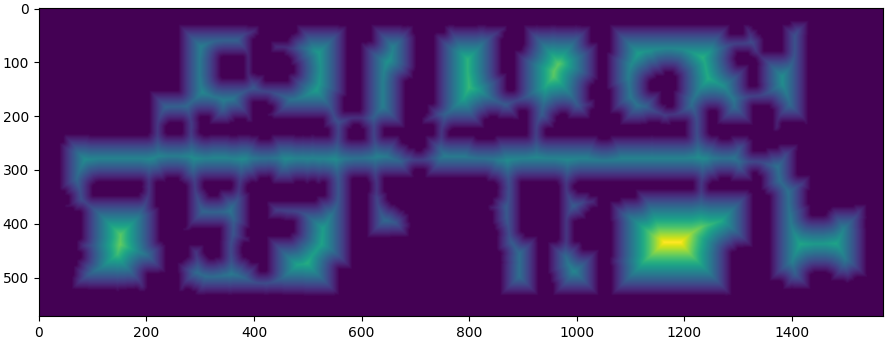
\includegraphics[width=\textwidth]{figures/50_implementation/ryu_distance_transform.png}
      \caption{Distance transform}
    \end{subfigure}%
    \begin{subfigure}{.5\textwidth}
      \centering
      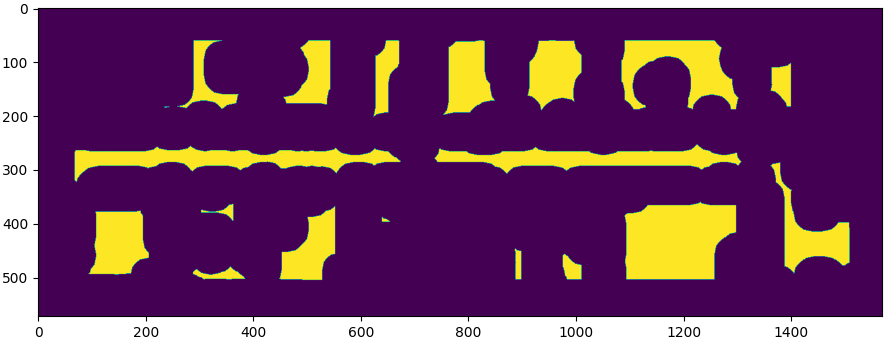
\includegraphics[width=\textwidth]{figures/50_implementation/ryu_markers.png}
      \caption{Markers as binary threshold of (a)}
    \end{subfigure}
    \caption[Distance transform and resulting markers]{Distance transform (a) and resulting markers (b) as initial information for the watershed algorithm.}
    \label{fig:distance_transform}
\end{figure}

To get the count, outlines and areas of each segment, the OpenCV function for detecting connected components is performed and returns a list of each area. With this list as input the watershed is then marker-controlled and provides a good segmentation of the whole floor into separate rooms as seen in Figure \ref{fig:watershed}.

\begin{figure}[h]
    \centering
    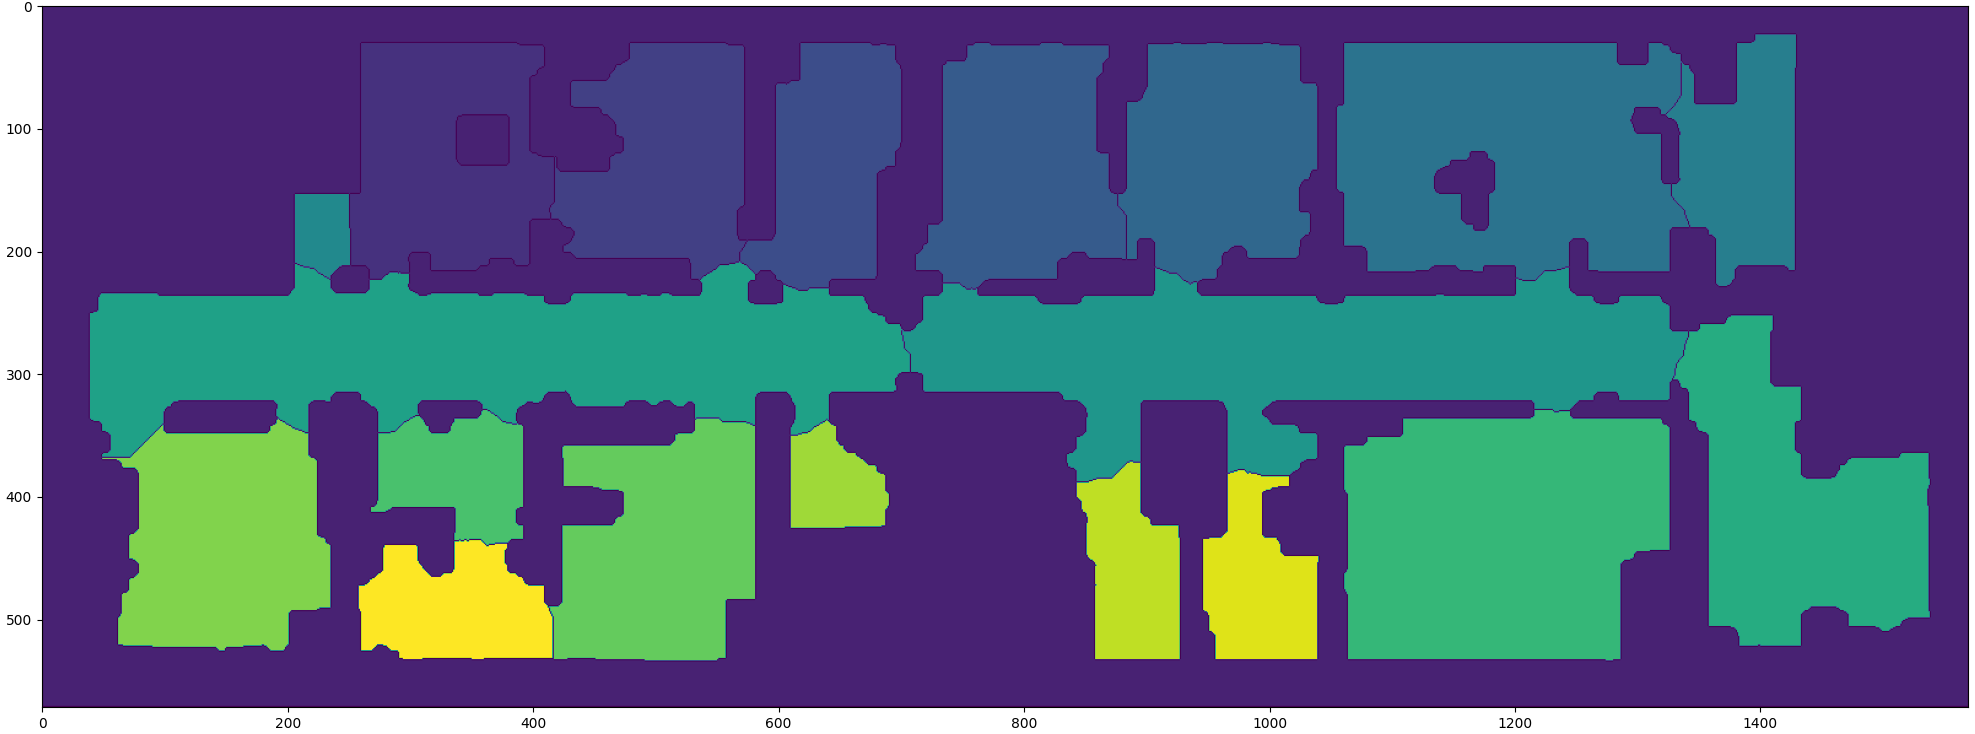
\includegraphics[width=0.75\textwidth]{figures/50_implementation/ryu_watershed.png}
    \caption[Marker-controlled watershed of the benchmark map]{Marker-controlled watershed of the benchmark map}
    \label{fig:watershed}
\end{figure}

This room segmentation provides the area for each room. To create a hierarchical graph from this the doors between them are important to create a hierarchical connection in the floor graph. The algorithm used in this work is based on the junction nodes extraction algorithm proposed by Ryu \cite{ryu_hierarchical_2020}. 

The base for this algorithm is the result of the watershed segmentation of Figure \ref{fig:watershed}. First, an adjacency matrix of the rooms are created. If rooms directly connect to each other with only a border created from the watershed in-between them, they have a real world connection. This connection and all pixels that lay on this border are stored. The distance transform from Figure \ref{fig:distance_transform} (a) is then taken to lookup the pixel with the maximum distance to the walls from that list of pixels on the border. Repeating this step for all connections in the adjacency matrix results in the bridge points with the maximum distance to the wall. 

\begin{figure}[h]
    \captionsetup[subfigure]{justification=centering}
    \centering
    \begin{subfigure}{.65\textwidth}
      \centering
      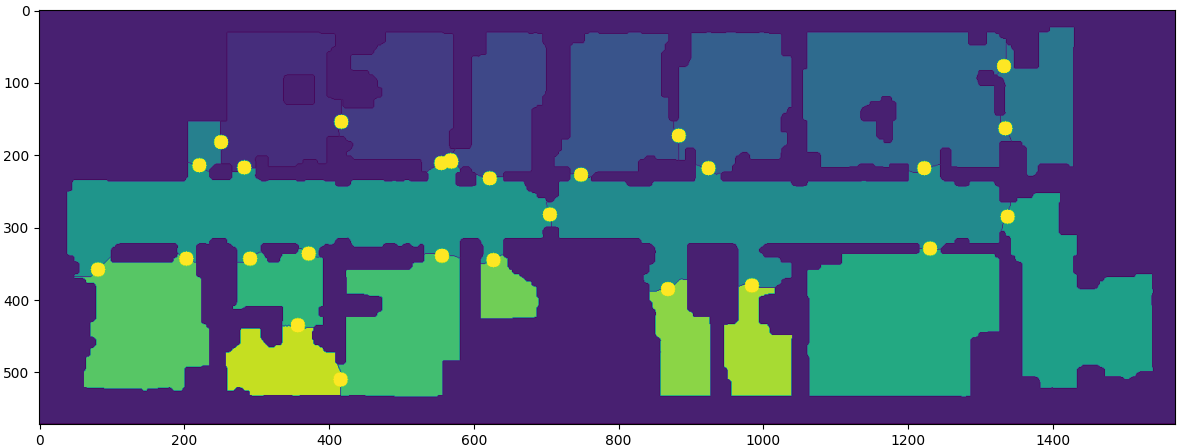
\includegraphics[width=\textwidth]{figures/50_implementation/ryu_bridge_nodes.png}
      \caption{Watershed result with detected bridge points}
    \end{subfigure}%
    \begin{subfigure}{.25\textwidth}
      \centering
      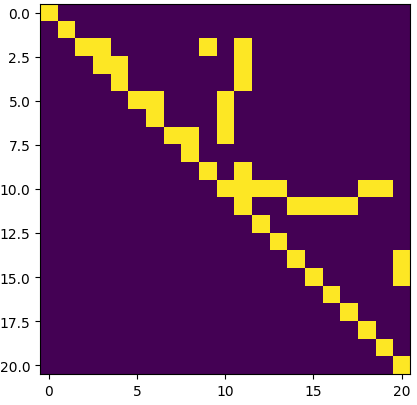
\includegraphics[width=\textwidth]{figures/50_implementation/ryu_adjacency_matrix.png}
      \caption{Adjacency matrix}
    \end{subfigure}
    \caption[The result of the bridge point detection algorithm]{The result of the bridge point detection algorithm. Bridge points overlayed on the segmented map (a). The adjacency matrix of the rooms (b). Rooms have always pixels connecting them to itself (diagonal line).}
    \label{fig:bridge_nodes}
\end{figure}

The segmented floor into rooms and their connections represented as bridge points can now be represented as a graph. Each room becomes a node in the floor graph. Each bridge point represents a door and becomes an edge in the graph. The corresponding graph can be seen in Figure \ref{fig:ryu_graph}. Note that this is inverted in the y-axis as all of the map previous images were taken from OpenCV which per default has its origin for images in the top left corner. In comparison, the graph representation is done with NetworkX which has its origin in the bottom left corner. 

\begin{figure}[h]
    \centering
    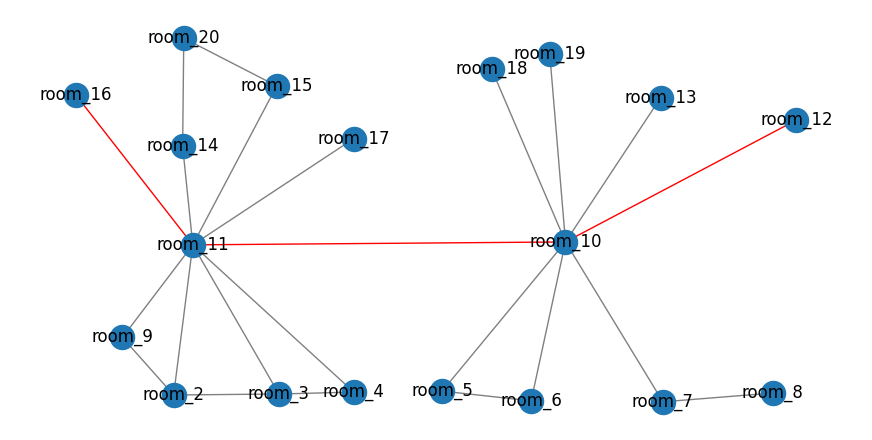
\includegraphics[width=0.7\textwidth]{figures/50_implementation/ryu_floor_graph.png}
    \caption[Graph representation of the benchmark map]{Graph representation of the benchmark map. Nodes are rooms and edges represent doors between them. In red is an example path from room 16 to room 12.}
    \label{fig:ryu_graph}
\end{figure}

To create an H-Graph for this benchmark, each room node has to hold a graph itself. These subgraphs are then the lowest hierarchical level and represent the roadmap of each room. Each Roadmap consits of collision free paths on the correspondign room-gridmap. To create this roadmap the straight path planner ILIR is used.


%% ==============================
\section{Roadmap Generation}
\label{sec:roadmap_generation}
%% ==============================
The first step for path planning is converting the environment in a Shapely object. This has the advantage, that basic shapes like lines, rectangles and polygons available, collision checks between these shapes are already implemented efficiently with a C library and the precision is higher than on the pixel based images. The images from OpenCV represent the environment in discrete pixels, this is helpful as the gridmap recorded from the laser scanners has exactly this resolution. However for collision checks and creating paths as lines it is important to precisely model these shapes. Lines should be one dimensional shapes which have no are. In comparison a line in an numpy matrix as used by OpenCV is represented in a row of pixels each with a certain width and height. This produces unexpected behavior and wrong results. The converted shapely environment can be seen in Figure \ref{fig:ryu_shapely}

\begin{figure}[h]
    \centering
    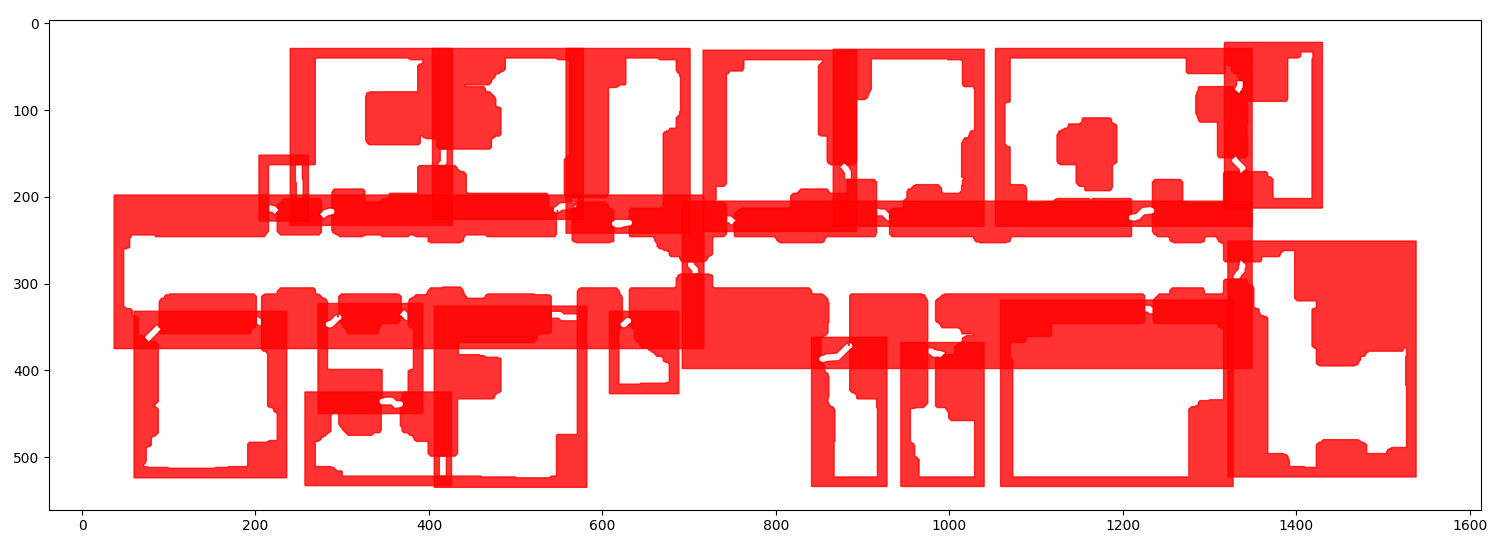
\includegraphics[width=0.75\textwidth]{figures/50_implementation/ruy_shapely.png}
    \caption[Shapely representation of the benchmark map]{Shapely representation of the benchmark map. Each room has its own environment and is surrounded by red obstacles. All room environments are drawn in one single image for visualization resulting in overlapped red obstacles.}
    \label{fig:ryu_shapely}
\end{figure}

In each room the largest interior rectangles are searched in an iterative process and combined to a polygon. The algorithm is from Marzeh et. al \cite{marzeh_algorithm_2019} and the used python implementation from Weber \cite{weber_largest_2023}. The proposed Iterative Largest Interior Rectangle (ILIR) algorithm extends these ideas by repeatedly searching the largest rectangle. Each rectangle is then subtracted from the original area and the same process is repeated with the remaining area. This produces not only the largest rectangle but also a polygon which is aligned to the axis of the coordinate frame. Just finding the largest interior polygon would not be useful as with high resolution this would just approximate the original shape. Also the edges of this polygon would not be parallel to the walls of the room which is an important requirement for the proposed algorithm. Additionally for each rectangle it is decided if the shape belongs more to a corridor or to a room based on predefined parameters. For an corridor the rectangle is collapsed to a straight line to provide a better path for the robot. In Algorithm \ref{lst:pseudo_code_ilir} the pseudo code of the ILIR straight path planner is shown.

\lstset{language=C++, mathescape=true, caption={Pseudo code of the ILIR straight path planner}, label={lst:pseudo_code_ilir}, morekeywords={from, to, is, input, output, each, in, end}}
\begin{lstlisting}[float=h]
input: gridmap, parameter
output: roadmap

room_list $\gets$ markerControlledWatershed(gridmap)

bridge_points $\gets$ extractBridgePoints(room_list)

for each room in room_list:

    while largest_contour.area > parameter.min_area:
    
        largest_contour $\gets$ maxContourByArea(room)
            
        largest_rectangle $\gets$ largestInteriorRectangle(largest_contour)

        if isCorridor(largest_rectangle):
            roadmap $\gets$ centerLine(largest_rectangle)
        else
            roadmap $\gets$ largest_rectangle

        room $\gets$ (room - largest_rectangle)
    end

    roadmap $\gets$ mergeRectangles(roadmap)
    
    roadmap $\gets$ connectBridgePoints(bridge_points)
end
\end{lstlisting}

In Figure \ref{fig:ilir_room_roadmap} the ILIR algorithm is applied on room 2 of the benchmark map. The red shapely environment represents the \(C\)-space for the path planning problem. The free area from (a) is converted into the \(C\)-space and a safety margin is applied with a dilation operation onto the walls and obstacles.  Therefor obstacles in the \(C\)-space look bigger than they are in the real world. This safety margin depends on the size of the robot and additional safety considerations. This allows to treat the robot as a dot in \(C\)-space and still ensure a collision free path. 

\begin{figure}[h]
    \captionsetup[subfigure]{justification=centering}
    \centering
    \begin{subfigure}{.31\textwidth}
      \centering
      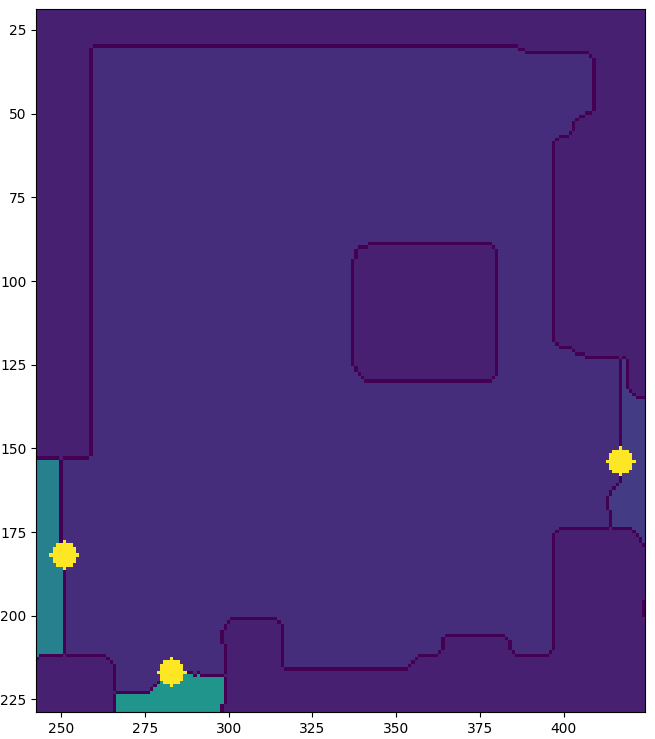
\includegraphics[width=\textwidth]{figures/50_implementation/ryu_room2_clean.png}
      \caption{Room after segmentation}
    \end{subfigure}%
    \begin{subfigure}{.33\textwidth}
      \centering
      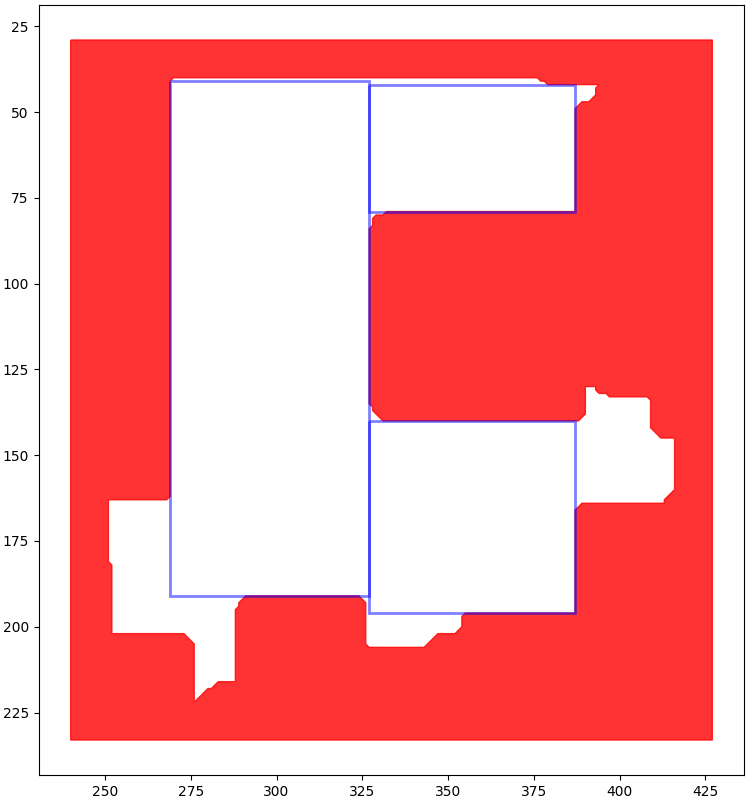
\includegraphics[width=\textwidth]{figures/50_implementation/ryu_room2_rectangles.png}
      \caption{largest interior rectangles}
    \end{subfigure}%
    \begin{subfigure}{.33\textwidth}
      \centering
      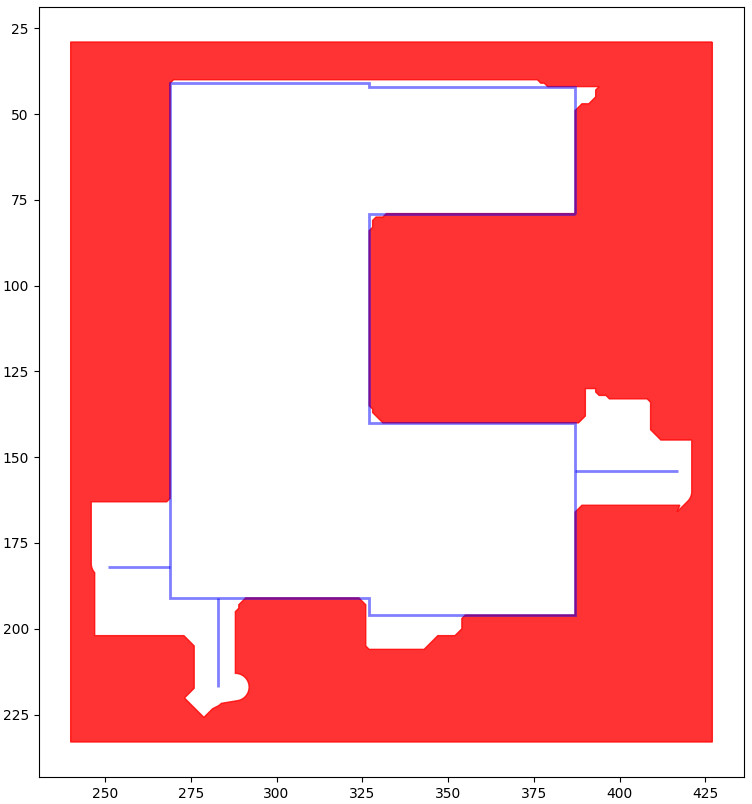
\includegraphics[width=\textwidth]{figures/50_implementation/ryu_room2_roadmap.png}
      \caption{Roadmap with ILIR}
    \end{subfigure}
    \caption[Application of the ILIR straight path planner on room 2 from the benchmark map]{Application of the ILIR straight path planner on room 2 from the benchmark map. The red obstacles are enlarged by the radius of the robot to ensure collision free paths.}
    \label{fig:ilir_room_roadmap}
\end{figure}
\todo{Add image of roadmap graph room2 and section in text abput it}

As the last step of the ILIR algorithm, the door of neighbouring rooms are connected to the merged rectangles. In Figure \ref{fig:ilir_room_roadmap} (a) three doors to other rooms can bee seen as yellow points. These are then connected to the polygon and form the resulting roadmap in (c). These connections are created first by checking the direct straight line with the shortest distance between the door and the roadmap. If this line is in collision, an A* search is done to find the shortest possible connections. This resulting path from A* will then be smoothed and turned into a series of straight lines which are then added to the roadmap. For the actual path planning in the real world, the robot can be at an random valid position in the room and first has to find a collision free path to the roadmap before it can follow the roadmap the door of the next room or an elevator of the next floor. This connection of start and goal positions that or not on the roadmap is done by the same process and can bee seen in the next chapter in Algorithm \ref{}. To make this roadmap searchable in a H-Graph it os converted to nodes and edges in the corresponding room graph (c). The connections in z-axis reoresent the hierarchical connections to another graph. They have no path cost and therefore will not be considered in the total distance of the path. By repeatedly applying the ILIR algorithm to each room in the previously segmented gridmap the levels H1 and H2 of the H-Graph can be automatically generated. In Figure \ref{fig:ryu_roadmap} a visualization of all the roadmaps of each room combined and overlayed on the image from the watershed is showed.

\begin{figure}[h]
    \centering
    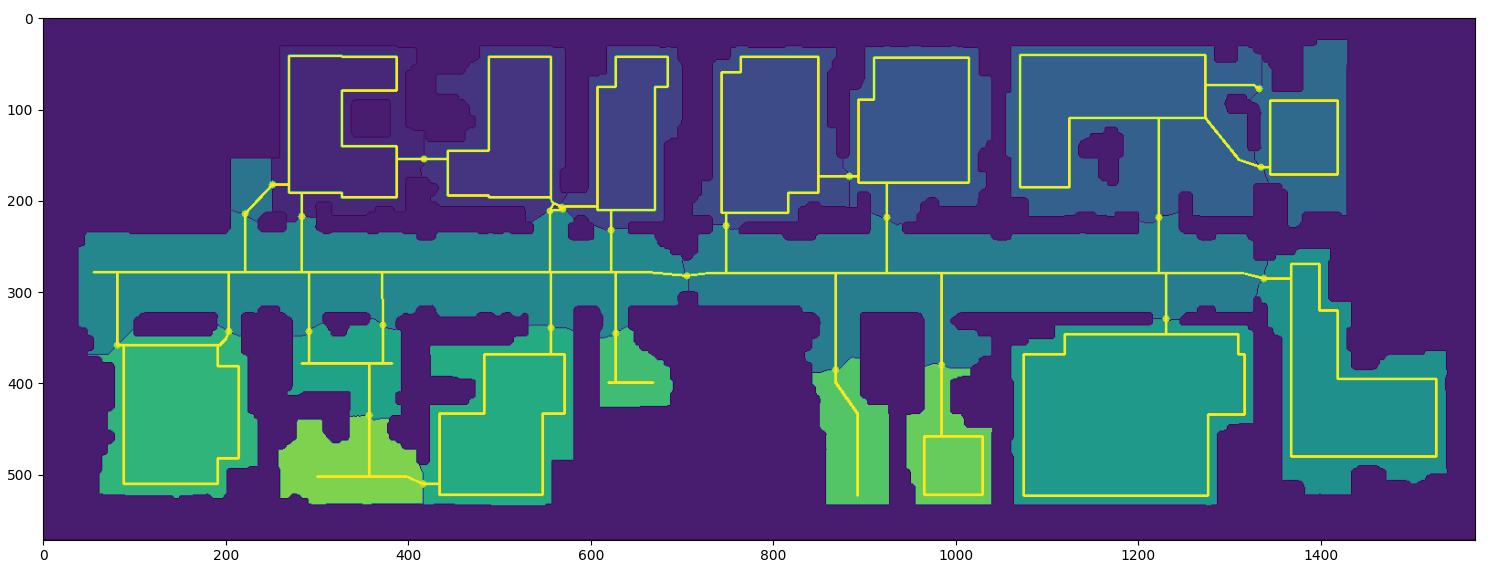
\includegraphics[width=0.75\textwidth]{figures/50_implementation/ryu_roadmap.png}
    \caption[Roadmap of the entire floor combined]{Roadmap of the entire floor combined and overlayed on the result from the watershed algorithm. It can be seen that paths in corridors are collapsed to a single line in the center.}
    \label{fig:ryu_roadmap}
\end{figure}

The ILIR algorithm is able to find a solution if a solution exists. This is ensured by the A* planner which is both complete and optimal. Thus the ILIR is also complete. However although the A* is used for bridge point connections the rest of the generated roadmap can not guarantee the shortest path. Thus the ILIR algorithm produces a path which is not optimal in terms of path length.

\todo{Zeitkomplexität}

%% ==============================
\section{Hierarchical Planning}
\label{sec:impl_hierarchical_planning}
%% ==============================


Pseudocode of recursive planning function


\lstset{language=python, mathescape=true, caption={Unique H-Graph positions and path representation}, label={lst:pseudo_code_ilir}, morekeywords={from, to, is, input, output, each, in, end}}
\begin{lstlisting}[float=h]
# general description of a unique position:
$p = \{p_{Hn}, p_{Hn-1}, ..., p_{H1}\}$

# specific unique position with 4 hierarchies in Python:
p_hierarchy = ["Building F", "Floor 2", "Room 2", (50,210)]

# specific example path with 4 hierarchies in Python:
path = {
    "Building F": {
        "Floor 3": {
            "Meeting Room": {},
            "Corridor": {},
            "Elevator": {},
            "Floor 2_Elevator_bridge": {}
        },
        "Floor 2": {
            "Floor 3_Elevator_bridge": {},
            "Elevator": {},
            "Corridor": {},
            "Terrace2": {},
            "Terrace_Floor 1_Ring F_bridge": {}
        },
        "Terrace_Floor 1_bridge": {}
    },
    "Terrace": {
        "Building F_Floor 2_bridge": {},
        "Floor 1": {
            "Building F_Floor 2_Terrace2_bridge": {},
            "Ring F": {}
        }
    }
}
\end{lstlisting}

\lstset{language=C++, mathescape=true, caption={Pseudo code of Hierarchical Path Planning}, label={lst:pseudo_code_ilir}, morekeywords={from, to, is, input, output, each, in, end}}
\begin{lstlisting}[float=h]
input: start_hierarchy, goal_hierarchy, h_graph
output: path

for hierarchy in [start_hierarchy, goal_hierarchy]:

    room, pos $\gets$ getHierarchyH2(hierarchy)
    
    if pos not in room.roadmap:
    
        if noCollision(straightLine(pos, room.roadmap)):
        
            path $\gets$ straightLine(pos, room.roadmap)
            
            room.roadmap $\gets$ path
        else:
            path $\gets$ A*Planner(pos, room.roadmap)
            
            room.roadmap $\gets$ path

path $\gets$ RecursiveHierarchicalPlanner(
            start_hierarchy, goal_hierarchy, h_graph)

\end{lstlisting}

Pseudocode of plan function with adding positions not on the roadmap

Time complexity of Dijstra and recursion

Mention Completness and Optimality


% https://stackoverflow.com/questions/13467674/determining-complexity-for-recursive-functions-big-o-notation

% Bounds of the running time of Dijkstra's algorithm on a graph with edges {{mvar|E}} and vertices {{mvar|V}} can be expressed as a function of the number of edges, denoted <math>|E|</math>, and the number of vertices, denoted <math>|V|</math>, using [[big-O notation]]. 
% The simplest version of Dijkstra's algorithm stores the vertex set {{mvar|Q}} as a linked list or array, and edges as an [[adjacency list]] or [[Adjacency matrix|matrix]]. In this case, extract-minimum is simply a linear search through all vertices in {{mvar|Q}}, so the running time is <math>\Theta(|E| + |V|^2) = \Theta(|V|^2)</math>.

% For [[sparse graph]]s, that is, graphs with far fewer than <math>|V|^2</math> edges, Dijkstra's algorithm can be implemented more efficiently by storing the graph in the form of adjacency lists and using a [[self-balancing binary search tree]], [[binary heap]], [[pairing heap]], or [[Fibonacci heap]] as a [[priority queue]] to implement extracting minimum efficiently. To perform decrease-key steps in a binary heap efficiently, it is necessary to use an auxiliary data structure that maps each vertex to its position in the heap, and to keep this structure up to date as the priority queue {{mvar|Q}} changes. With a self-balancing binary search tree or binary heap, the algorithm requires
% :<math>\Theta((|E| + |V|) \log |V|)</math>
% time in the worst case (where <math>\log</math> denotes the binary logarithm <math>\log_2</math>); for connected graphs this time bound can be simplified to <math>\Theta( | E | \log | V | )</math>.  The [[Fibonacci heap]] improves this to
% :<math>\Theta(|E| + |V| \log|V|).</math>

%% ==============================
\section{Multi-Floor Navigation with Behavior Trees}
\label{sec:multi_floor_behavior_trees}
%% ==============================

BaseMovement ROS2 Action interface for move base.

Trick to set mapframe to target floor to give information fpr hierarchical planning.

Pseudocode or interface of the cpp plugin

Behavior tree for multi floor navigation



%% ==============================
\chapter{Results}
\label{sec:results}
%% ==============================
The results of this work are the straight path planner ILIR, the hierarchical planning algorithm, and the planner plugin for integration into ROS 2. In this chapter, these approaches are evaluated and compared with related work. The evaluation criteria have been presented in Chapter \ref{sec:methods} "Methods".

%% ==============================
\section{Comparison of Straight Path Planners}
\label{sec:evaluation_straight_path}
%% ==============================
The evaluation of the planner algorithm ILIR is done on the benchmark maps of Ryu \cite{ryu_hierarchical_2020} and Hou et al. \cite{hou_straight_2021}. And to specifically show the effects of public space disturbance, the second room of the first map and the ninth room of the second map were chosen. The metrics and the calculation of the number of paths used on each map were presented in Chapter \ref{sec:methods}. For better readability, a complete list is repeated here:

\begin{enumerate}
    \item \textbf{Success Rate}: Percentage of valid paths found
    \item \textbf{Path Length}: Total length from start to goal in pixels
    \item \textbf{Planning Time}: Total planning time including smoothing
    \item \textbf{Path Smoothness}: Sum of deviation angles divided by path length
    \item \textbf{Obstacle Clearance}: Mean distance from path to obstacles
    \item \textbf{Distance Deviation}: Standard deviation of distance between path and obstacles
    \item \textbf{Distance to Centroid}: Mean distance of the path to the centroid of the room
    \item \textbf{Disturbance of Public Space}: Largest open area within the map divided by total room area (details in Chapter \ref{sec:new_metric})
\end{enumerate}

The different planners that will be compared to the ILIR algorithm are listed below. These planners were chosen because they are widely used in the field of path planning for robotics and provide a good baseline for comparison. In addition, A* can be considered the ground truth for the shortest path distance since it is complete and optimal. The other two represent the different approach of probabilistic sampling.

\begin{enumerate}
    \item \textbf{ILIR}: Iterative Largest Interior Rectangle
    \item \textbf{A*}: A* Planner
    \item \textbf{PRM}: Probabilistic Roadmap
    \item \textbf{RRT}: Rapidly Exploring Random Tree
\end{enumerate}

\begin{figure}[h]
    \captionsetup[subfigure]{justification=centering}
    \centering
    \begin{subfigure}{.25\textwidth}
      \centering
      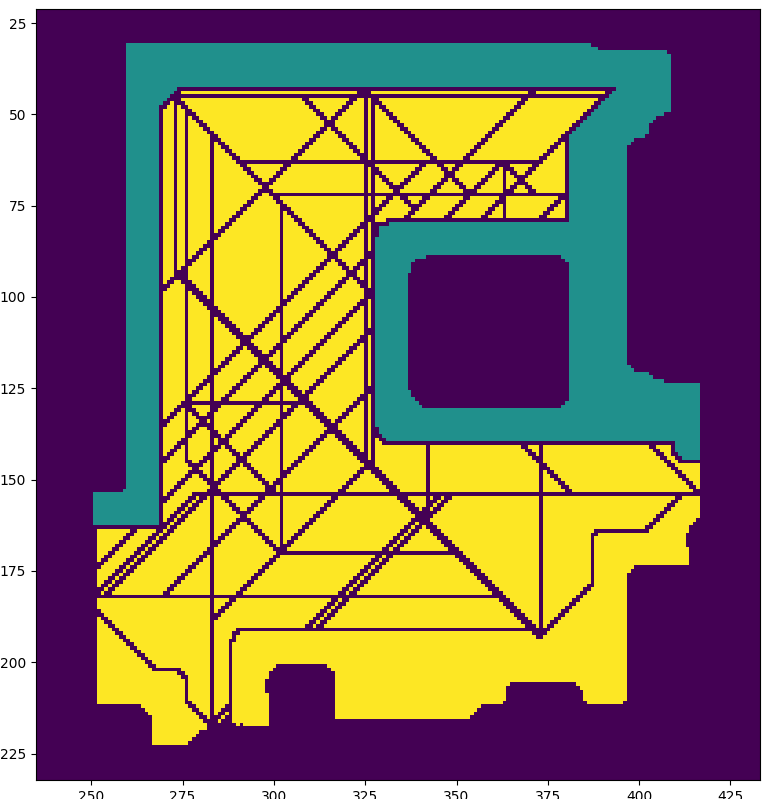
\includegraphics[width=\textwidth]{figures/60_results/room2_disturbance_astar_unsmoothed.png}
      \caption{A*}
    \end{subfigure}%
    \begin{subfigure}{.24\textwidth}
      \centering
      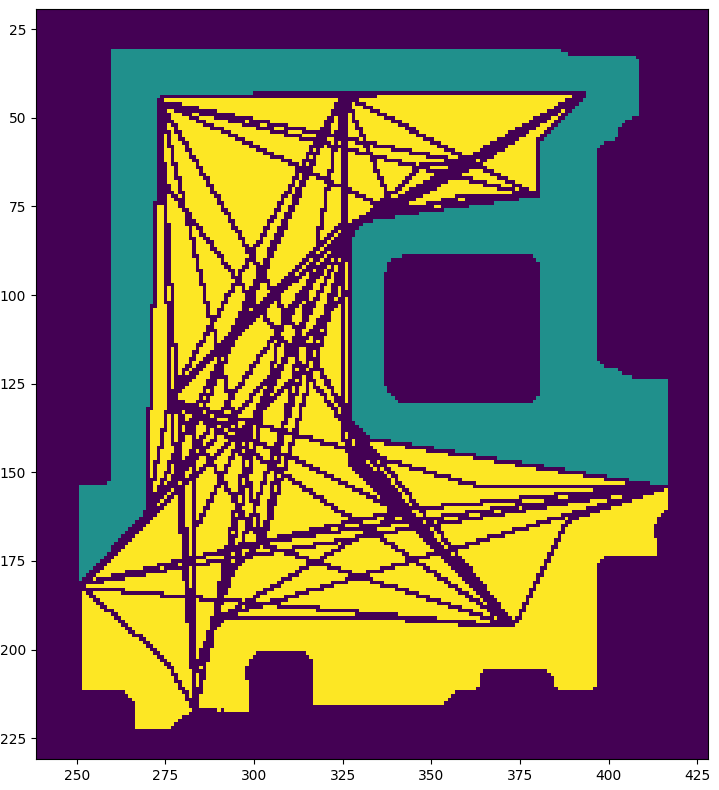
\includegraphics[width=\textwidth]{figures/60_results/room2_disturbance_astar_smooth.png}
      \caption{A* smoothed}
    \end{subfigure}
    \caption[Comparison of A* with and without smoothing algorithm]{Comparison of A* with and without smoothing algorithm. Turquoise and yellow areas are both representing the original room map.}
    \label{fig:smoothing}
\end{figure}

The first step for a fair comparison is to smooth the output path of each planner as it would realistically be used by a robot for driving. This is necessary because the A*, for example, produces paths on a gridmap that has a certain resolution. This leads to "steps" for diagonal lines. And there are always many possible solution paths with exactly the same length. It is only determined by the order of node expansion by the specific implementation. To force the path to take the most direct route, unnecessary nodes are removed and the more direct connection is chosen. Figure \ref{fig:smoothing} shows the effect of this smoothing. The same is done for PRM and RRT. Both planners create a roadmap by sampling random points in the environment. This roadmap is then connected and provides a path. This is not optimal because there are many unnecessary turns. For smoothing, the nodes with the highest deviation angles between the incoming and outgoing lines are tried to be removed. If this is possible, the surrounding nodes are connected directly and the process is repeated until no node can be removed because it would result in a collision path. This is not done for the ILIR, because it would contradict the goal of leaving the middle for undisturbed human traffic.

\begin{figure}[h]
    \captionsetup[subfigure]{justification=centering}
    \centering
    \begin{subfigure}{.25\textwidth}
      \centering
      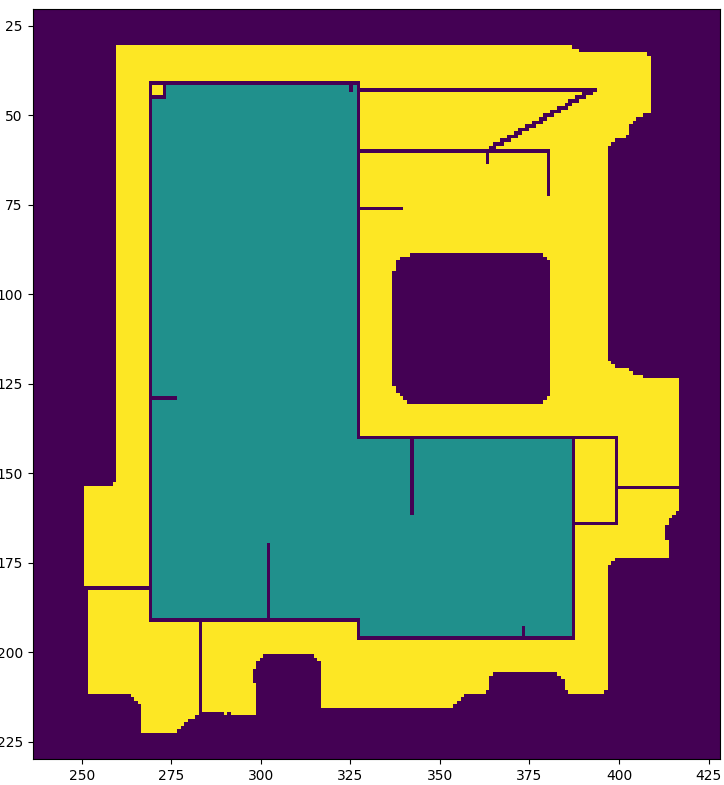
\includegraphics[width=\textwidth]{figures/60_results/room2_disturbance_ilir.png}
      \caption{ILIR}
    \end{subfigure}%
    \begin{subfigure}{.25\textwidth}
      \centering
      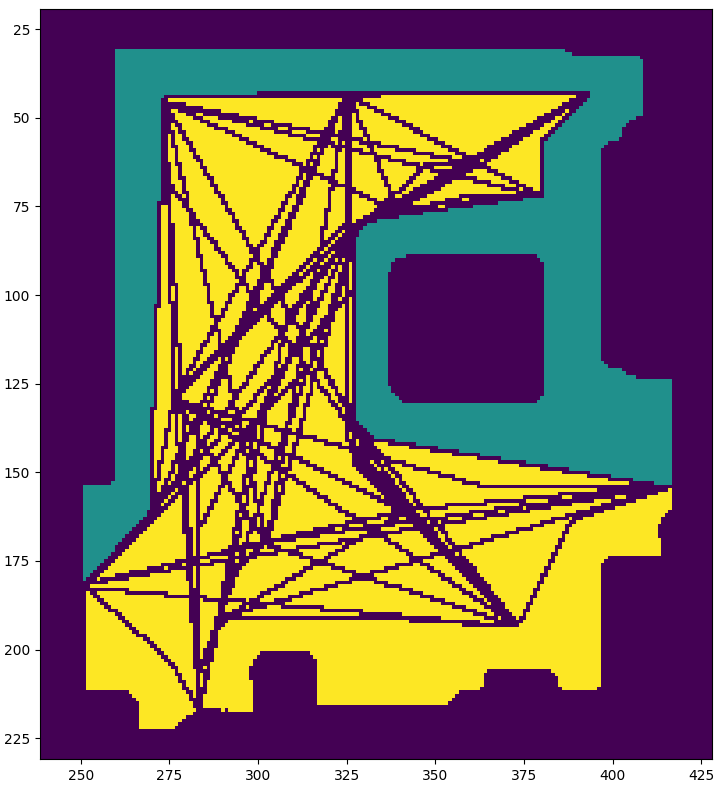
\includegraphics[width=\textwidth]{figures/60_results/room2_disturbance_astar.png}
      \caption{A*}
    \end{subfigure}%
    \begin{subfigure}{.25\textwidth}
      \centering
      \includegraphics[width=\textwidth]{figures/60_results/room2_disturbance_prm.png}
      \caption{PRM}
    \end{subfigure}%
    \begin{subfigure}{.25\textwidth}
      \centering
      \includegraphics[width=\textwidth]{figures/60_results/room2_disturbance_rrt.png}
      \caption{RRT}
    \end{subfigure}
    \caption[Comparison of planning methods on room 2 of benchmark map 1]{Comparison of planning methods on room 2 of benchmark map 1 with 78 paths. The turquoise area is the largest free area where no path is crossing and the combination with yellow is the original room map.}
    \label{fig:ryu_room2_comparison}
\end{figure}

Figure \ref{fig:ryu_room2_comparison} shows the comparison of smoothed paths in the second room of the first benchmark map. It can be clearly seen that the ILIR planner forces the paths onto its roadmap and keeps the inner area free. In the figure, the metric for public space disturbance is represented visually by the colors of the background: the turquoise area is the largest free area where no path crosses, and the remaining area is yellow. The calculation of this metric is explained in Chapter \ref{sec:methods} with the formula \ref{equ:disturbance}.

\begin{table}[ht]
\centering
\begin{tabular}{lc|cccc}
\hline
\textbf{Metric} & \textbf{Unit} & \textbf{ILIR} & \textbf{A*} & \textbf{PRM} & \textbf{RRT} \\
\hline
Success rate & -                & \textbf{1.000}          & \textbf{1.000}          & \textbf{1.000}      & 0.987 \\
Mean planning time & s          & \textbf{0.002} & 1.094         & 0.879     & 0.014 \\
Mean path length & px           & 204.4          & \textbf{118.8} & 136.3    & 131.5 \\
Mean smoothness & °/px          & 1.296         & \textbf{0.203} & 0.241    & 0.214 \\
Mean obstacle clearance & px    & \textbf{14.4} & 22.5          & 25.4      & 25.4 \\
Std obstacle clearance & px     & \textbf{4.1}  & 5.9           & 5.7       & 5.9 \\
Mean distance to centroid & px  & \textbf{70.0}          & 56.6          & 57.7      & 56.3 \\
Disturbance of public space & - & \textbf{0.443} & 0.698          & 0.663      & 0.664 \\
\hline
\end{tabular}
\caption{Comparison of planning methods on room 2 of benchmark map 1 with 78 paths}
\label{tab:room2_results}
\end{table}

Table \ref{tab:room2_results} shows the results of the evaluation for each planner. The room 2 represents an average room that could appear on most floors in an office environment. It is only about ~8x6 m in size. But already in this small room the differences between the planners are visible. Due to its geometrically built roadmap compared to expanding single nodes over the entire coordinate space, ILIR is the fastest with 2 ms, followed by RRT with 14 ms. This is an improvement of 86 \%. Note that the ILIR's roadmap creation time occurs during the room segmentation and is not included here. In terms of path length, as expected, the A* planner has the shortest path and ILIR has the longest since it avoids the middle area. The smoothness is a factor that is surprisingly bad for ILIR with 2.37 °/px. It was expected that by forcing straight paths the resulting path would be smoother. But this is a false conclusion, as it has more 90° turns than the others. This adds up to a large total turn angle and cannot be compensated by the longer path. The obstacle clearance of ILIR is low, which is not necessarily a bad thing as it shows that the paths are closer to the wall. The standard deviation of this distance shows that these paths are also more consistent than the others. The metric of the distance to the centroid of the room also shows that the paths of ILIR do not go directly through the center. This means that the paths are close to the walls and are generally less fluctuating than the paths of the other planners. Finally, the custom metric for the disturbance of the room space shows that ILIR has the lowest disturbance with 44.3 \%, which is 22 \%-points better than the next best. This proves that the ILIR planner achieves its goal of planning paths that are straight and do not disturb the human working area even in a small room. Also in Figure \ref{fig:ryu_room2_comparison} it can be clearly seen that the paths are deterministic and always follow the same roadmap. This makes them more predictable for humans.

\begin{figure}[h]
    \captionsetup[subfigure]{justification=centering}
    \centering
    \begin{subfigure}{.35\textwidth}
      \centering
      \includegraphics[width=\textwidth]{figures/60_results/room9_disturbance_ilir.png}
      \caption{ILIR}
    \end{subfigure}%
    \begin{subfigure}{.35\textwidth}
      \centering
      \includegraphics[width=\textwidth]{figures/60_results/room9_disturbance_astar.png}
      \caption{A*}
    \end{subfigure}
    \begin{subfigure}{.35\textwidth}
      \centering
      \includegraphics[width=\textwidth]{figures/60_results/room9_disturbance_prm.png}
      \caption{PRM}
    \end{subfigure}%
    \begin{subfigure}{.35\textwidth}
      \centering
      \includegraphics[width=\textwidth]{figures/60_results/room9_disturbance_rrt.png}
      \caption{RRT}
    \end{subfigure}
    \caption[Comparison with common planners on room 9 of benchmark map 2]{Comparison with common planners on room 9 of benchmark map 2 with 171 paths. The turquoise area is the largest free area where no path is crossing and the combination with yellow is the original room map.}
    \label{fig:hou_room9_comparison}
\end{figure}

\begin{table}[h]
\centering
\caption{Comparison of planning methods on room 9 of benchmark map 2 with 171 paths}
\label{tab:room9_results}
\begin{tabular}{lc|cccc}
\hline
\textbf{Metric}                    & \textbf{Unit} & \textbf{ILIR} & \textbf{AStar} & \textbf{PRM} & \textbf{RRT} \\
\hline
Success rate                       & -    & \textbf{1.000}          & \textbf{1.000}         & 0.632          & 0.942 \\
Mean planning time                 & s    & \textbf{0.141} & 8.077         & 0.962          & 0.783 \\
Mean path length                   & px   & 496.3          & \textbf{256.8}& 262.0          & 304.6 \\
Mean smoothness                    & °/px & 1.374          & 0.248         & \textbf{0.205} & 0.245 \\
Mean obstacle clearance            & px   & \textbf{15.2}  & 45.0          & 53.5           & 53.1  \\
Std obstacle clearance             & px   & \textbf{9.1}   & 17.6          & 18.0           & 19.9 \\
Mean distance to centroid          & px   & \textbf{175.7}          & 134.6         & 126.3          & 128.9  \\
Disturbance of public space        & -    & \textbf{0.166} & 0.951         & 0.921          & 0.887 \\
\hline
\end{tabular}
\end{table}

For comparison, the same metrics are now applied to a conference lobby that is much larger (~30x50 m) and has more entrances. Figure \ref{fig:hou_room9_comparison} shows this room. The corresponding result of the evaluation is shown in Table \ref{tab:room9_results}. For this benchmark, the ILIR planner is again the fastest in terms of planning time with 0.141 s per path. The mean obstacle clearance, its standard deviation, and the distance to the centroid again show that ILIR's paths are closer to the walls and less fluctuating. The difference in the disturbance of the public space is even greater, and with more than 72 \%-points apart and a total of 16 \% of the room area occupied by potential paths of the robot, it leaves enough space for human activities.

In the previous evaluation, some rooms were highlighted to demonstrate the planner's capabilities on an average map as well as for an extreme case. But of course most of the robot's paths are through corridors. Especially there the goal property of straight paths is important to avoid collisions with people and to establish a predictable behavior. For this reason, the focus of the following evaluation is on the straight paths and the general appearance, and not on the path-specific metrics. 

\begin{figure}[h]
    \captionsetup[subfigure]{justification=centering}
    \centering
    \begin{subfigure}{.5\textwidth}
      \centering
      \includegraphics[width=\textwidth]{figures/60_results/hou2_roadmap_RGVG.png}
      \caption{RGVG \cite{beeson_towards_2005}}
    \end{subfigure}%
    \begin{subfigure}{.5\textwidth}
      \centering
      \includegraphics[width=\textwidth]{figures/60_results/hou2_roadmap_evg.png}
      \caption{EVG \cite{beeson_towards_2005}}
    \end{subfigure}
    \begin{subfigure}{.5\textwidth}
      \centering
      \includegraphics[width=\textwidth]{figures/60_results/hou2_roadmap_htm.png}
      \caption{HTM \cite{hou_straight_2021}}
    \end{subfigure}%
    \begin{subfigure}{.5\textwidth}
      \centering
      \includegraphics[width=\textwidth]{figures/60_results/hou2_roadmap_ilir.png}
      \caption{ILIR}
    \end{subfigure}
    \caption[Comparison with related work on room 9 of benchmark map 2]{Comparison with related work on room 9 of benchmark map 2. The roadmap is drawn in blue, red and yellow, obstacles are black and dark purple}
    \label{fig:hou_comparison}
\end{figure}

Figure \ref{fig:hou_comparison} shows the complete benchmark map 2 and the roadmaps generated by the Reduced General Voronoi Graph (RGVG), the Extended Voronoi Graph (EVG) \cite{beeson_towards_2005}, the Hierarchical Topological Map (HTM) \cite{hou_straight_2021} and the ILIR planner (this work). It can be seen that the EVG in \ref{fig:hou_comparison} (b), which is configured with a sensory horizon of 1.5 m, always stays close to the wall if there is a larger room. If not, it stays in the middle of the corridor. However, it suffers from strong jitter caused by sensor noise. The paths in the corridor are not straight and not good for driving a robot. The HTM approach (c) solves the straight path problem for the corridor well, but struggles in larger rooms. The paths are straight but almost never parallel to the walls and go straight through the open space. The ILIR planner (d) solves both problems by providing straight paths in the middle of each corridor, while staying close and parallel to the walls in large open areas. Since the implementations of the other approaches are not open source, it was not possible to directly compare these paths with specific metrics.

%% ==============================
\section{Comparison of Hierarchical Planners}
\label{sec:evaluation_hierarchical}
%% ==============================
The hierarchical planner should be compared to other implementations from related work using a common set of benchmarks. Since such a common set of benchmarks does not exist, and the planners from related work are not open source, this evaluation for the entire n-level H-Graph is done only as a proof of concept. However, the SIRRT* algorithm by Ryu \cite{ryu_hierarchical_2020} uses the same benchmark map 1 and also implements a hierarchical planner, although only for two levels of hierarchy. Figure \ref{fig:ryu_floor_comparison} shows a comparison between SIRRT* and the proposed hierarchical planner combined with the roadmap from ILIR. Note that the SIRRT* planner is limited to two levels of hierarchy, as its focus is only on improving the speed of calculating paths in huge floors. 

\begin{figure}[h]
    \captionsetup[subfigure]{justification=centering}
    \centering
    \begin{subfigure}{0.75\textwidth}
      \centering
      \includegraphics[width=\textwidth]{figures/60_results/ryu_example_path_htm.png}
      \caption{SIRRT* \cite{ryu_hierarchical_2020}}
    \end{subfigure}
    \begin{subfigure}{0.75\textwidth}
      \centering
      \includegraphics[width=\textwidth]{figures/60_results/ryu_example_path_ilir.png}
      \caption{Hierarchical Planner using ILIR (this work)}
    \end{subfigure}
    \caption[Comparison of hierarchical planning on benchmark map 1]{Comparison of hierarchical planning on benchmark map 1}
    \label{fig:ryu_floor_comparison}
\end{figure}

The proposed hierarchical planner (b) uses the H-Graph to efficiently plan at the room level first and then searches only the corresponding roadmaps of these rooms. Since these roadmaps can be precomputed, a new search can be performed very quickly. In comparison, SIRRT* performs an RRT search in each room for each path. This could also be speeded up by caching the roadmap, but is not described in \cite{ryu_hierarchical_2020}. The problem of choosing the correct room door for connections where two or more doors lead to the same room is solved by both planners. This can be seen in (a) between room 16 and room 10. As well as in (b) on the same rooms. The shortest path inside room 16 would be to connect to the first door on the left, but this would lead to a longer overall path. 

\begin{figure}[h]
    \centering
    \includegraphics[width=\textwidth]{figures/40_concept/ltc_graph_complete.png}
    \caption[Graph of the IRAS campus for evaluation]{Graph of the IRAS campus for evaluation. All the room level nodes are drawn in the same graph just for visualization.}
    \label{fig:ltc_graph_complete}
\end{figure}

To further test the capabilities of the proposed hierarchical planner, a model of the \gls{iras} research campus is created, see Figure \ref{fig:ltc_graph_complete}. It can be verified that the hierarchical planner is able to plan between arbitrary paths in this complex environment. The built H-Graph has 4 hierarchy levels and a total of 4,454 nodes, the exact number on each hierarchy level can be seen in Table \ref{tab:ltc_graph_nodes}. Note that the total number of nodes on each level includes bridge nodes. Also, the gridmap for each of these rooms has not been recorded. With an estimated average room size of 8x10m, the resulting total number of cells in the gridmaps is 1,672,000 pixels. If all of these cells were searched by a regular planar path planner such as A*, the advantages of the H-Graph and hierarchical planning become obvious.

\begin{table}[ht]
\centering\captionsetup{justification=centering}
\begin{tabular}{ccc}
\hline
\textbf{Level} & \textbf{Name} & \textbf{Number of nodes} \\
\hline
4 & Buildings & 7 \\
3 & Floors & 58\\
2 & Rooms & 209  \\
1 & Nodes on roadmap & 4180  \\
0 & Cells in gridmap & 1,672,000  \\
\hline
\end{tabular}
\caption{Total number of nodes in the H-Graph of the IRAS campus}
\label{tab:ltc_graph_nodes}
\end{table}

%% ==============================
\section{Evaluation in Simulation}
\label{sec:evaluation_simulation}
%% ==============================
To validate the developed concept, it is tested in a simulated hospital environment. The environment was previously presented in Figure \ref{fig:aws_hospital} in Chapter \ref{sec:simulation}. Amazon has made its "AWS RoboMaker Hospital World" \cite{aws_robotics_aws_2023} open source, but has not published any research done with it. This means that it was not possible to compare this approach with related work in the area of multi-floor navigation in the same environment. However, there is a work by Fredriksson et al. \cite{fredriksson_semantic_2023} that uses the same hospital simulation from Amazon, but focuses on detecting semantic features such as intersections and corridors. It also aims to provide a clean roadmap for the robot's global navigation. Figure \ref{fig:aws_comparison} shows a comparison of this approach and the resulting roadmap with the proposed planner and other related work like EVG and RGVG.

\begin{figure}[h]
    \captionsetup[subfigure]{justification=centering}
    \centering
    \begin{subfigure}{.5\textwidth}
      \centering
      \includegraphics[width=\textwidth]{figures/60_results/aws_roadmap_rgvg.png}
      \caption{RGVG}
    \end{subfigure}%
    \begin{subfigure}{.5\textwidth}
      \centering
      \includegraphics[width=\textwidth]{figures/60_results/aws_roadmap_evg.png}
      \caption{EVG}
    \end{subfigure}
    \begin{subfigure}{.5\textwidth}
      \centering
      \includegraphics[width=\textwidth]{figures/60_results/aws_roadmap_semantic.png}
      \caption{Semantic \cite{fredriksson_semantic_2023}}
    \end{subfigure}%
    \begin{subfigure}{.5\textwidth}
      \centering
      \includegraphics[width=\textwidth]{figures/60_results/aws_roadmap_horizontal.png}\vspace{5pt}
      \caption{ILIR}
    \end{subfigure}
    \caption[Comparison of planning methods for the hospital simulation]{Comparison of planning methods for hospital simulation. For (c), semantic features are colored: Green for paths, brown for intersections, blue for dead ends, and pink for paths to a new frontier. In (d) the segmented rooms are colored with an increasing color palette, the roadmap is yellow.}
    \label{fig:aws_comparison}
\end{figure}

With this roadmap generated by ILIR \ref{fig:aws_comparison} (d), the complete multi-floor navigation with ROS 2 can be tested. Note that the simulation environment has two floors, but they are duplicates of each other with the same layout. Figure \ref{fig:aws_neobotix_simulation} shows the \gls{rviz} (left) and the Gazebo simulation (right). RVIZ represents all the data the robot knows about the environment. It does not matter to the robot if this data comes from a simulation or from sensors in the real world. The robot used in this simulation is the MPO\_500 from Neobotix, because the same planners of this robot are also used in the PeTRA project. The robot can be seen in RVIZ as well as in the lower floor on the left side (the ceiling is transparent). It emits blue rays from the laser scanner just for visualization. The goal for this proof of concept is the elevator on the left. In RVIZ, the path from the hierarchical planner on the ILIR roadmap can be seen as a thin red line. There is also a smaller blue line that represents the current motion of the controller keeping the robot on the path. This is also used to smoothly navigate around the sharp corners in the red roadmap. The goal given by the hierarchical planner is determined by the H-Graph as the shortest path from the bottom floor to the top floor. The location of the elevators on the map was previously marked when the graph was created. When the robot reaches the elevator, it is teleported to the top floor in the simulation and is given a new path to the final goal on the top floor. Once the final goal is reached, another multi-floor navigation with its own behavior tree is triggered to bring the robot back down to the bottom floor. This behavior was successfully tested 10 times in a loop. This proves the capability of the developed multi-floor navigation system.

\begin{figure}[h]
    \centering
    \includegraphics[width=\textwidth]{figures/60_results/aws_neobotix_simulation.png}
    \caption[UML diagram of the H-Graph implementation]{UML diagram of the H-Graph implementation. Blue components were taken from the community, green components were developed in this work.}
    \label{fig:aws_neobotix_simulation}
\end{figure}

Finally the multi-floor navigation system was tested on the real robot. Due to a problem with PeTRA using an old version of the Navigation stack implemented in ROS 1 and the lack of time, not all components can be demonstrated on the real robot. However single components have been tested and work as planned with the current system. This is for example the whole structure of a multi-floor planning request coordinated with the BT.
\begin{figure}[H]
    \centering\captionsetup{justification=centering}
    \includegraphics[width=0.6\textwidth]{figures/60_results/petra_elevator.png}
    \caption[The real PeTRA robot in the elevator mock-up]{The real PeTRA robot in the elevator mock-up}
    \label{fig:petra_elevator}
\end{figure}
\noindent
This has been successfully tested and used for navigation in the lab with mock-ups for a potential elevator. A lot of work has also been done in a student project to enable PeTRA to push elevator buttons with its integrated robotic arm. This solves the problem of changing floors where no WLAN interface is available. With these components it was successfully demonstrated that the PeTRA system can perform a multi-floor navigation task in a mock-up environment as shown in Figure \ref{fig:petra_elevator}, where the elevator was simulated by a cardboard box and the floor remained the same. The straight path planner could not be integrated into ROS 1 because it would require a lot of parameter fine-tuning to get the associated path controller to work as expected.

%% ==============================
\chapter{\iflanguage{ngerman}{Diskussion}{Discussion}}
\label{sec:discussion}
%% ==============================

\dots
%% ==============================
\chapter{\iflanguage{ngerman}{Zusammenfassung und Ausblick}{Conclusion}}
\label{sec:conclusion}
%% ==============================

\dots

\Bibliography{\mybibliographyfiles}

% \addmybibentry
%% appendix.tex
%%

%% ==============================
\Appendix
\label{ch:Appendix}
%% ==============================


\section{First Appendix Section}
\label{sec:app-first-sections}



\begin{figure} [ht]
  \centering
   ein Bild
  \caption{A figure}
  \label{fig:Beispiela}
\end{figure}


\section{Second Appendix Section}
\label{sec:app-second-sections}



\begin{figure} [ht]
  \centering
   ein Bild
  \caption{A figure}
  \label{fig:Beispielb}
\end{figure}

\dots


\includedeclaration

\end{document}
